\documentclass[a4paper,12pt]{article}
\usepackage[french]{babel}
\usepackage{hyperref}
\usepackage{csquotes}
\usepackage{geometry}
\usepackage{graphicx}
\usepackage{listings}
\usepackage{hyperref}
\usepackage{float}
\usepackage{appendix}
\usepackage{xcolor}
\usepackage{colortbl}
\usepackage{tabularx}
\usepackage{array}
\usepackage[utf8]{inputenc}
\usepackage[T1]{fontenc}
\usepackage[numbers]{natbib}
\usepackage{placeins} % for \FloatBarrier because of the images in Agenda Rétrospectif
\geometry{top=2cm, bottom=2cm, left=2cm, right=2cm}

\definecolor{CornflowerBlue}{RGB}{100,149,237}  % For functional needs
\definecolor{RoyalBlue}{RGB}{65,105,225}   % For non-functional needs
\definecolor{MediumAquamarine}{RGB}{102,205,170} % For validation strategy

\lstdefinelanguage{pseudocode}{
    morekeywords={procedure,if,then,else,while,do,return,for,each,in,begin,end},
    sensitive=false,
    morecomment=[l]{//},
    morestring=[b]",
}

\lstset{
    language=pseudocode,
    basicstyle=\ttfamily,
    keywordstyle=\color{blue}\bfseries,
    commentstyle=\color{gray},
    stringstyle=\color{red},
    breaklines=true,
    frame=single,
    captionpos=b
}

\begin{document}

\begin{titlepage}
    \centering
    \vspace*{1cm}
    {\huge\bfseries Jeu de plateau: Othello}
    \vspace{3cm}

    {Matis Duval, Rémy Heuret, Lucas Marques, Gabriel Tardiou}
    \vspace{2cm}

    {\scshape\small Université de Bordeaux\\}
    \vspace{1cm}
    {\scshape\small Projet de Programmation, Master 1}
    \vspace{1cm}

    \vfill
    {\large Avril 2025}
\end{titlepage}

\newpage

\tableofcontents

\newpage

\section{Présentation de l'existant}

Selon la Fédération francaise d’Othello, sur sa page \textit{Histoire}, le jeu
d’Othello que l’on connaît aujourd’hui est une version modifiée du jeu Reversi,
créé autour de 1880, supposément par Lewis Waterman ou John W.
Mollett.\cite{FFOthelloHistoire} Reversi lui-même étant une variante du jeu
Annexation créé en 1870 par J. W. Mollett – la seule différence étant le
plateau de jeu: une croix de 10 par 4 pour
Annexation\cite{TameTheBoardGameAnnexation}, et un carré de 8 par 8 pour
Reversi. Ces deux personnes d’origine anglaise se disputent l’invention du jeu,
et ont créé deux versions différentes : Reversi Waterman\footnote{Image prise
    sur le site de la Fédération Française d’Othello.
    \url{https://www.ffothello.org/images/histoire/jeux-anciens/reversi_waterman-1880.jpg}}
et Reversi Mollett\footnote{Image prise sur le site de la Fédération Française
    d’Othello.
    \url{https://www.ffothello.org/images/histoire/jeux-anciens/reversi_mollett-1880.jpg}}.\\

\begin{figure}[h]
    \centering
    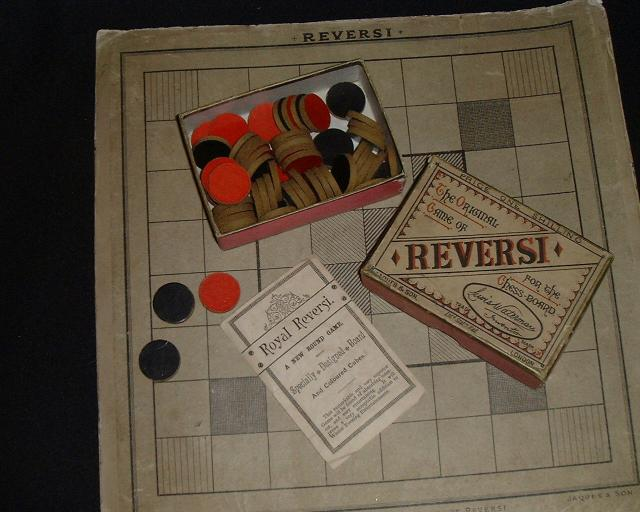
\includegraphics[width=0.5\textwidth]{images/reversi_waterman-1880.jpg}
    \caption{Jeu Reversi, version Lewis Waterman .\\
        Le jeu comporte un papier représentant le plateau, un livret de règles, et des pions.}
    \title{fig:Jeu Reversi, version Lewis Waterman.}

    \centering
    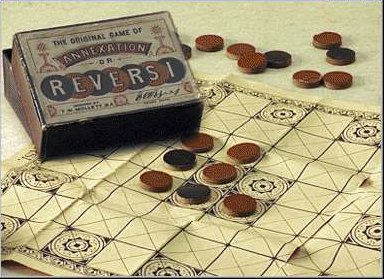
\includegraphics[width=0.5\textwidth]{images/reversi_mollett-1880.jpg}
    \caption{Jeu Reversi, version J. W. Mollett.\\
        Le jeu comporte un plateau en papier et des pions.}
    \title{fig:Jeu Reversi, version J. W. Mollett.}
\end{figure}

Ce jeu de plateau était très apprécié vers la fin du 19\up{ème} siècle, surtout
en Angleterre. Un article sur le jeu parut en 1888 dans un magazine spécialisé
dans les jeux de dames.\\ \newpage On retrouve des éditions aux États-Unis,
ainsi qu’en Europe Centrale, et des livres de stratégie sont créés.\\ Le jeu
Reversi perd de sa popularité au 20\up{ème} siècle, jusqu’en 1971, où un
Japonais du nom de Goro Hasegawa réinvente et redistribue le jeu sous un autre
nom : Othello. Le père de Goro Hasegawa, un professeur de littérature anglaise,
lui propose le nom d’Othello en référence à la pièce de W. Shakespeare, en
raison de ses nombreux retournements de situation.\\ Le jeu devient rapidement
populaire, et la première compétition est organisée en 1973, soit deux ans
après la commercialisation du jeu.\\ Dès 1976, Othello est arrivé en Angleterre
et aux États-Unis, et les premiers championnats du monde d’Othello se tiennent
en 1977, et reviennent tous les ans.\\ Les règles d’Othello diffèrent
légèrement de celles de Reversi. Désormais, on fixe la position initiale des
pions, et il est possible de prendre des pions (non placés sur le plateau) à
son adversaire lorsque celui-ci passe son tour.\\ En France, le jeu se
popularise à partir de la fin des années 1970, et la Fédération Française
d’Othello (FFO) est créée en 1983. La FFO met régulièrement à jour son
calendrier des prochains tournois sur sa page \textit{Prochains tournois et
    évènements}.\cite{FFOthelloTournois} \footnote{Image prise sur le site de la
    Fédération Française d’Othello.
    \url{https://www.ffothello.org/images/histoire/jeux-modernes/othelloroyal.jpg}}.\\

\begin{figure}[h]
    \centering
    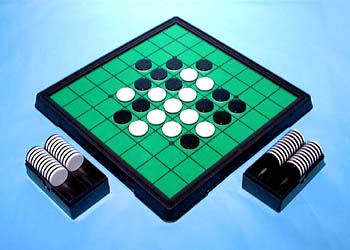
\includegraphics[width=0.5\textwidth]{images/othelloroyal.jpg}
    \caption{Jeu Othello, Othello Royal distribué par Tsukada.\\
        Jeu utilisé en tournois en France.}
    \title{fig:Jeu Reversi, version J. W. Mollett.}
\end{figure}

Les règles en tournoi, spécifiquement, pour les championnats du monde d’Othello
(World Othello Championships – WOC) sont décrites dans le document World
Othello Championships Rules, publié en septembre 2019 par la Fédération
Mondiale d’Othello (World Othello Federation – WOF).\cite{WOCRules2023}\\ Les
championnats du monde se tiennent annuellement, et déterminent le champion des
catégories Individuels, Femmes, et Jeunes.\\ La compétition se tient sur trois
jours. Pendant les deux premiers jours, le rang est déterminé par des matchs à
temps limité, en rondes Suisses ou Robin, puis les demi-finales et la finale se
tiennent le troisième jour.\\ Seulement les équipes des nations membres de la
WOF peuvent participer.\\ Les règles sont très spécifiques quant à
l’éligibilité des joueurs, le compte des scores, et l’organisation du tournoi.
Les procédures pour l’édition des listes de classement, ou en cas de matériel
défectueux, d’égalité y sont également décrites très précisément.\\ \newpage Le
site de la Fédération Mondiale d’Othello tient à jour un calendrier
\footnote{Calendrier international des tournois d'Othello, régulièrement mis à
    jour par la Fédération Mondiale d'Othello.
    \url{https://www.worldothello.org/calendar}} des prochains tournois organisés
sur leurs pages liées aux tournois: \textit{World Othello Championship} et
\textit{Othello calendar}.\cite{WOFCalendar}\cite{WOCTournaments}\\ Des
championnats européens se tiendront le 31 mai et 1er juin de cette année, à
Prague en République Tchèque.\\ Le prochain championnat du monde aura lieu à
Ankara en Turquie, en novembre 2025, et réunira plus de 84 pays.\\

Le jeu d’Othello est relativement populaire, on en trouve fréquemment en clubs
de jeux de société ou jeux de plateau.\\ Il est également possible de jouer en
ligne sur des sites, recommandés par la FFO sur leur page \textit{Jouer sur
    internet}.\cite{FFOthelloJouerInternet} \footnote{Guide des plateformes en
    ligne pour jouer à Othello, recommandé par la Fédération Française d'Othello.
    \url{https://www.ffothello.org/communaute/jouer-sur-internet/}} Les plus
populaires cités sont PlayOK\cite{PlayOKReversi} \footnote{Site PlayOK offrant
    la possibilité de jouer au Reversi en ligne contre des adversaires du monde
    entier, avec système de classement. \url{https://www.playok.com/fr/reversi/}},
qui propose des parties en ligne ; et eOthello \footnote{Plateforme eOthello
    permettant de jouer gratuitement à Othello en différé.
    \url{https://www.eothello.com/}} pour jouer plusieurs parties en différé, avec
72 heures de temps limite par coup.\\ Le site PlayPager\cite{PlayPagerOthello}
\footnote{Plateforme PlayPager permettant de jouer gratuitement à
    Othello/Reversi en ligne contre l'ordinateur ou d'autres joueurs.
    \url{https://playpager.com/othello-reversi/}} permet de jouer à deux joueurs ou
contre une intelligence artificielle sur un plateau en 8 par 8.\\ La Fédération
Française d’Othello propose également de se mettre en relation avec des joueurs
via une liste de diffusion.\\ Il existe aussi des serveurs discord tels que
Othello Academy \footnote{Serveur Discord "Othello Academy" regroupant une
    communauté active de joueurs, des tutoriels et des tournois amicaux.
    \url{https://discord.me/othelloacademy}}, ou encore Board Games Geek sur
lequels des joueurs peuvent se rencontrer, discuter du jeu et de stratégie.\\

\newpage

\section{Règles du jeu}

Othello se joue sur un plateau unicolore de 64 cases : l’\textit{othellier}. \\
Les cases de l’othellier sont notées avec les lettres de A à H pour les
colonnes et les chiffres de 1 à 8 pour les lignes. \\ Chaque joueur possède 64
pierres, de couleur blanche sur une face et noire sur l’autre.

\vspace{0.4cm}

Avant que la partie ne commence, 4 pierres sont déposées sur l'othellier : 2
pierres noires en \texttt{E4} et \texttt{D5}, et 2 pierres blanches en
\texttt{E5} et \texttt{D4}.

\begin{figure}[h]
    \centering
    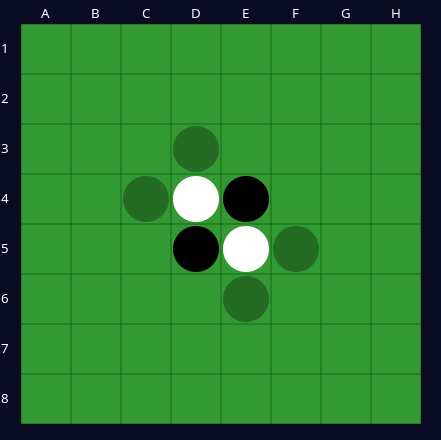
\includegraphics[width=0.5\textwidth]{images/othello_rules_start.png}
    \caption{Position de départ de l'othellier.}
    \title{fig:Début de partie.}
\end{figure}

\vspace{0.4cm}

Le but du jeu est de terminer la partie en ayant plus de pierres de sa couleur
que celle de l’adversaire sur l’othellier. \\ Au début de la partie, les
joueurs noir et blanc sont désignés. Chaque joueur doit poser ses pierres sur
l’othellier avec la face de sa couleur visible.

\vspace{0.4cm}

Les joueurs jouent à tour de rôle, en commençant par le joueur noir. \\ Un tour
désigne une pierre posée de sorte à capturer au minimum une pierre adverse.

\vspace{0.4cm}

Pour capturer une (ou plusieurs) pierres, il faut positionner de part et
d’autre des pierres adverses une pierre de sa propre couleur, sur une même
ligne, colonne ou diagonale. \\ Toutes les pierres ennemies capturées sont
alors retournées, pour que la face visible soit de la couleur du joueur qui a
initié la capture. \\

\vspace{0.4cm}

Il faut noter qu’une capture ne peut être initiée qu’à partir de la pierre qui
vient d’être posée. \\ Il ne peut donc pas y avoir de réaction en chaîne. \\ Si
la pierre posée permet de capturer dans plusieurs directions, alors toutes les
pierres doivent être capturées, peu importe la direction.

\vspace{0.4cm}

\newpage

Voici un exemple de capture : \\

Les noirs souhaitent jouer le coup \texttt{C6}. On regarde alors dans toutes
les directions en partant de cette pierre s'il y a des pierres blanches prises
en "sandwich" par pierres noires. Les pierres \texttt{C5} et \texttt{D5} sont
donc les 2 pierres capturées.

\begin{figure}[h]
    \centering
    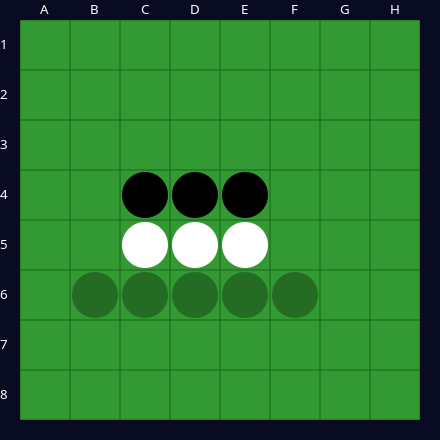
\includegraphics[width=0.5\textwidth]{images/othello_rules_before_move.png}
    \caption{Coups possibles par le joueur noir.}
    \title{fig:Coups possibles noirs.}
\end{figure}

\begin{figure}[h]
    \centering
    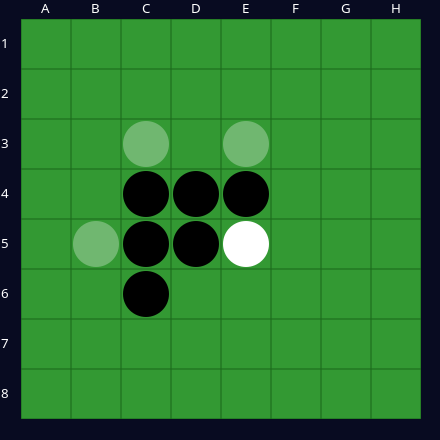
\includegraphics[width=0.5\textwidth]{images/othello_rules_after_move.png}
    \caption{Capture des pierres \texttt{C5} et \texttt{D5} par le joueur noir.}
    \title{fig:Capture noire.}
\end{figure}

La partie peut se terminer de deux manières :
\begin{itemize}
    \item L’othellier est complètement rempli (64 pierres posées).
    \item Les deux joueurs n’ont plus de coup possible.
\end{itemize}

\vspace{0.2cm}

Une fois la partie terminée, on compte le nombre de pierres possédées par
chaque joueur. Le joueur possédant le plus de pierres remporte la partie. \\

Les règles se fient à celles de la FFO (Fédération Française d'Othello
\cite{FFOthelloRegles}).\\

Afin d’établir des stratégies, les joueurs doivent avoir en tête certains
concepts clés, décrits très clairements sur le site de la FFO, aux pages
\textit{Principes stratégiques} et \textit{Comment jouer les ouvertures}.
\cite{FFOthelloStrategie}\cite{FFOthelloOuvertures} Ils proposent également un
livret d'initiation au jeu en format pdf, coécrit par la FFO et Emmanuel
Lazard.\cite{FFOthelloLivret}\\

Tout d’abord, il faut se rappeler que le nombre de pièces de chaque joueur peut
changer rapidement au cours de la partie. Il est important de placer des
pierres stables, qui ne pourront pas être capturées.\\ Ensuite, placer ses
pions dans les coins garantit souvent les pièces autour comme stables. Le
joueur essaiera de ne pas jouer dans les cases proches des coins pour ne pas
les donner à son adversaire.\\ Il faut tenter de réduire le plus possible les
options de son adversaire, tout en essayant d’avoir beaucoup de choix de son
côté.\\ Calculer le nombre de cases restantes permet de se projeter sur la fin
de partie, et de qui des deux joueurs va placer le dernier pion. Comme le
résultat est calculé à partir du dernier état du jeu, jouer en dernier peut
faire une différence. On peut calculer ses prochains coups en conséquence,
essayer de faire passer son tour à son adversaire, ou l’inciter à jouer sur
certaines cases.\\

\newpage

\section{Descriptions des algorithmes et structures de données}

Nous utilisons des \texttt{Bitboards} pour représenter l’état du plateau –
modulo le joueur courant qui est un membre de l’énumération \texttt{Color}.\\
Nous nous basons sur le fonctionnement des entiers en Python, pouvant être de
taille arbitrairement longue, pour encoder nos plateaux sur un seul entier.\\
On linéarise notre plateau, autrement dit, on le représente en dimension 1
comme si l’on représentait une image dans un tableau à une dimension.\\ En
regardant les bits composant notre nombre, on peut savoir si une case est
occupée ou non, selon si le bit à la position de cette case est à 1 ou non.\\

Étant donné la simplicité du plateau — à savoir que chaque joueur a des pions
tous identiques — il n’est nécessaire d’utiliser que deux \texttt{bitboards}
pour représenter l’état du plateau de jeu : un pour les pions noirs et un pour
les pions blancs.\\ On peut, à partir de ces deux \texttt{bitboards}, modéliser
tout le plateau.\\

Par exemple, l’ensemble des cases occupées serait l’union des pions noirs et
blancs.\\ On peut également utiliser les propriétés des opérations bit à bit
pour appliquer les algorithmes du jeu d’Othello efficacement, en travaillant
sur l’ensemble du plateau à la fois.\\

\begin{lstlisting}[caption={Pseudocode pour l'initialisation des bitboards : classe BitboardProperties}, label={lst:bitboard_properties}]
class BitboardProperties:
  static instances := empty map
  // instance variables: size, mask, west_mask, east_mask
  // will be set in the get() method

  static method get(size):
  if size not in instances:
    // create a new instance
    structure := new BitboardProperties()
    structure.size := size
    structure.mask := 0
    structure.west_mask := 0
    structure.east_mask := 0

    // compute the masks
    for i from 0 to (size * size - 1):
      structure.mask := structure.mask OR (1 shifted left by i)
      if i mod size = 0:
        structure.west_mask := structure.west_mask OR (1 shifted left by i)
      if i mod size = size - 1:
        structure.east_mask := structure.east_mask OR (1 shifted left by i)
    instances[size] := structure
  return instances[size]
\end{lstlisting}

\newpage

Nous nous sommes servis de l'article de Cameron Browne: \textit{Bitboard
    methods for games}\cite{BitboardMethods} pour mieux comprendre les bitboards et
leur utilisation, ainsi que les algorithmes qui les utilisent.\\

\vspace{0.5cm}

Pour la partie calcul des coups, nous utilisons l’algorithme \texttt{Line Cap
    Moves}, présenté dans \textit{Bitboard Methods for Games}, par Cameron Browne
(cité plus haut) :\\ Cet algorithme permet de générer un ensemble de coups
possibles dans chaque direction. C’est-à-dire, donner les emplacements pour
lesquels le joueur courant pourrait capturer des pions adverses dans une
direction à la fois.\\

D’abord, un ensemble de coups vide est créé, puis on itère sur toutes les
directions :\\ Nord, Nord-Est, Est, Sud-Est, Sud, Sud-Ouest, Ouest,
Nord-Ouest.\\ Ensuite, on génère un ensemble de cases \textit{candidates} par
intersection entre les pions ennemis et les pions amis \texttt{shift} de 1 dans
la direction courante.\\ Tant que cet ensemble de cases n’est pas vide, on
effectue les opérations suivantes :\\ L’ensemble de coups est actualisé en
ajoutant l’intersection entre l’ensemble vide, et les cases candidates
\texttt{shift} de 1 dans la direction.\\ Puis l’ensemble des cases candidates
est réécrit en l’intersection entre lui-même \texttt{shift} de 1 dans la
direction courante, et les pions adverses.\\ Lorsque l’ensemble de cases
candidates est vide, on peut changer de direction et recommencer. Et quand
toutes les directions ont été explorées, l’ensemble de coups contient tous les
coups possibles et légaux.\\ Afin de changer les pions capturés dans la couleur
du joueur courant, nous avons créé un algorithme en se basant sur l’algorithme
\texttt{Line Cap Moves} ci-dessus.\\ En partant de la case sur laquelle le
dernier pion a été placé, on se déplace sur tous les pions ennemis en les
retournant pour changer leur couleur.\\

\begin{lstlisting}[caption={Pseudocode pour l'algorithme line\_cap\_move\ : fonction CalculatePossibleMoves}, label={lst:calculate_possible_moves}]
function CalculatePossibleMoves(playerPieces, opponentPieces, emptySquares):
  possibleMoves := empty set
  directions := [North, NorthEast, East, SouthEast, South, SouthWest, West, NorthWest]

  for each direction in directions:
    // find candidate squares
    candidateSquares := opponentPieces AND (playerPieces shift by 1 in direction)
    while candidateSquares is not empty:
      possibleMoves := possibleMoves OR (emptySquares AND (candidateSquares shift by 1 in direction))
      // update candidate squares
      candidateSquares := (candidateSquares shift by 1 in direction) AND opponentPieces

  return possibleMoves
\end{lstlisting}

\newpage

Afin de changer les pions capturés dans la couleur du joueur courant, nous
avons créé un algorithme en se basant sur l’algorithme \texttt{Line Cap Moves}
ci-dessus.\\ En partant de la case sur laquelle le dernier pion a été placé, on
se déplace sur tous les pions ennemis en les retournant pour changer leur
couleur.\\ Tout d’abord, on récupère le dernier pion placé par le joueur
courant, puis on itère dans toutes les directions : Nord, Nord-Est, Est,
Sud-Est, Sud, Sud-West, West, Nord-West.\\ On \texttt{shift} le pion de 1 dans
la direction courante, le pion est donc un pion maintenant Ennemi.\\ Tant que
le pion n’est pas un pion Ami (pion de la couleur du joueur courant), on
effectue les opérations suivantes :\\ Le pion est changé de Ennemi à Ami : on
retourne le pion pour que sa couleur soit celle du joueur courant.\\ Puis on
\texttt{shift} le pion de 1 dans la direction courante.\\ Lorsque le pion sur
lequel on s’est déplacé est un pion Ami, on peut changer de direction et
recommencer.\\ Et quand toutes les directions ont été explorées, tous les pions
à capturer ont été changés en pions du joueur courant.\\

\begin{lstlisting}[caption={Pseudocode pour l'algorithme de capture de pions : FlipCapturedPieces}, label={lst:flip_captured_pieces}]
function FlipCapturedPieces(board, lastMovePlayed, currentPlayer):
  // starting position : last piece placed
  startPosition := lastMovePlayed
  directions := [North, NorthEast, East, SouthEast, South, SouthWest, West, NorthWest]

  for each direction in directions:
    // move one step in the current direction
    currentPosition := Shift(startPosition, direction, 1)

    if board[currentPosition] is opponent's piece:
      // store positions that might need to be flipped
      piecesToFlip := empty list

      // keep moving in this direction as long as we find opponent pieces
      while board[currentPosition] is opponent's piece:
        piecesToFlip.Add(currentPosition)
        currentPosition := Shift(currentPosition, direction, 1)

      // if we found a friendly piece at the end, flip all in between
      if board[currentPosition] is currentPlayer's piece:
        for each position in piecesToFlip:
          board[position] := currentPlayer's piece
\end{lstlisting}

\newpage

Nous avons également implémenté un \texttt{popcount} en utilisant l’algorithme
\texttt{SWAR}, décrit dans l'article de Sanjoy Das: \textit{A SWAR Algorithm
    for Popcount}\cite{SWARPointers}, sur des blocs de 64 bits, qui fonctionne sur
la base d’un diviser pour mieux régner sur des mots de 64 bits, permettant de
faire le \texttt{popcount} efficacement, ainsi qu’un algorithme permettant de
récupérer les positions à \texttt{1} dans le \texttt{bitboard} efficacement.\\

\begin{lstlisting}[caption={Pseudocode pour le popcount (implémentation de l'algorithme SWAR): PopCount}, label={lst:popcount}]
function PopCount(bits):
  summed := 0
  remainingBits := bits

  while remainingBits > 0:
    // Process each 64-bit chunk
    chunk := remainingBits AND 0xFFFFFFFFFFFFFFFF

    // Apply SWAR algorithm with progressive bit masking and shifting
    chunk := (chunk AND 0x5555555555555555) + ((chunk >> 1) AND 0x5555555555555555)
    chunk := (chunk AND 0x3333333333333333) + ((chunk >> 2) AND 0x3333333333333333)
    chunk := (chunk AND 0x0F0F0F0F0F0F0F0F) + ((chunk >> 4) AND 0x0F0F0F0F0F0F0F0F)
    chunk := (chunk AND 0x00FF00FF00FF00FF) + ((chunk >> 8) AND 0x00FF00FF00FF00FF)
    chunk := (chunk AND 0x0000FFFF0000FFFF) + ((chunk >> 16) AND 0x0000FFFF0000FFFF)
    chunk := (chunk AND 0x00000000FFFFFFFF) + ((chunk >> 32) AND 0x00000000FFFFFFFF)

    summed := summed + chunk
    remainingBits := remainingBits >> 64

  return summed
\end{lstlisting}

\newpage

Notre IA utilise deux algorithmes d’exploration de l’arbre des coups possibles
: \texttt{Minimax} et \texttt{Alpha-Beta pruning}.\\

L’algorithme \texttt{Minimax} est un algorithme qui, à partir d’un
\texttt{board} donné en entrée, crée un arbre de tous les coups possibles à une
profondeur définie. Il explore récursivement tous les coups possibles jusqu’à
arriver à une feuille de l’arbre.\\ Pour chaque feuille de l’arbre, un score
est calculé en utilisant une heuristique qui permet d’évaluer l’état d’un
plateau en considérant différentes caractéristiques.\\ Il remonte ensuite les
scores en alternant les coups "ami", qui cherchent à obtenir le meilleur score,
et les coups "ennemis", qui cherchent à obtenir le pire score.\\
\texttt{Minimax} renvoie le meilleur score atteignable depuis le \texttt{board}
donné en entrée.\\ \\ Dans l'exemple ci-dessous, on peut voir que les scores
des feuilles remontent en alternant les coups "ami" et "ennemi" (choisissant
respectivement le meilleur et le pire score). Minimax renvoit donc 19, qui est
le meilleur score atteignable depuis le plateau initial si les 2 joueurs jouent
les meilleurs coups théoriques.

\begin{figure}[h]
    \centering
    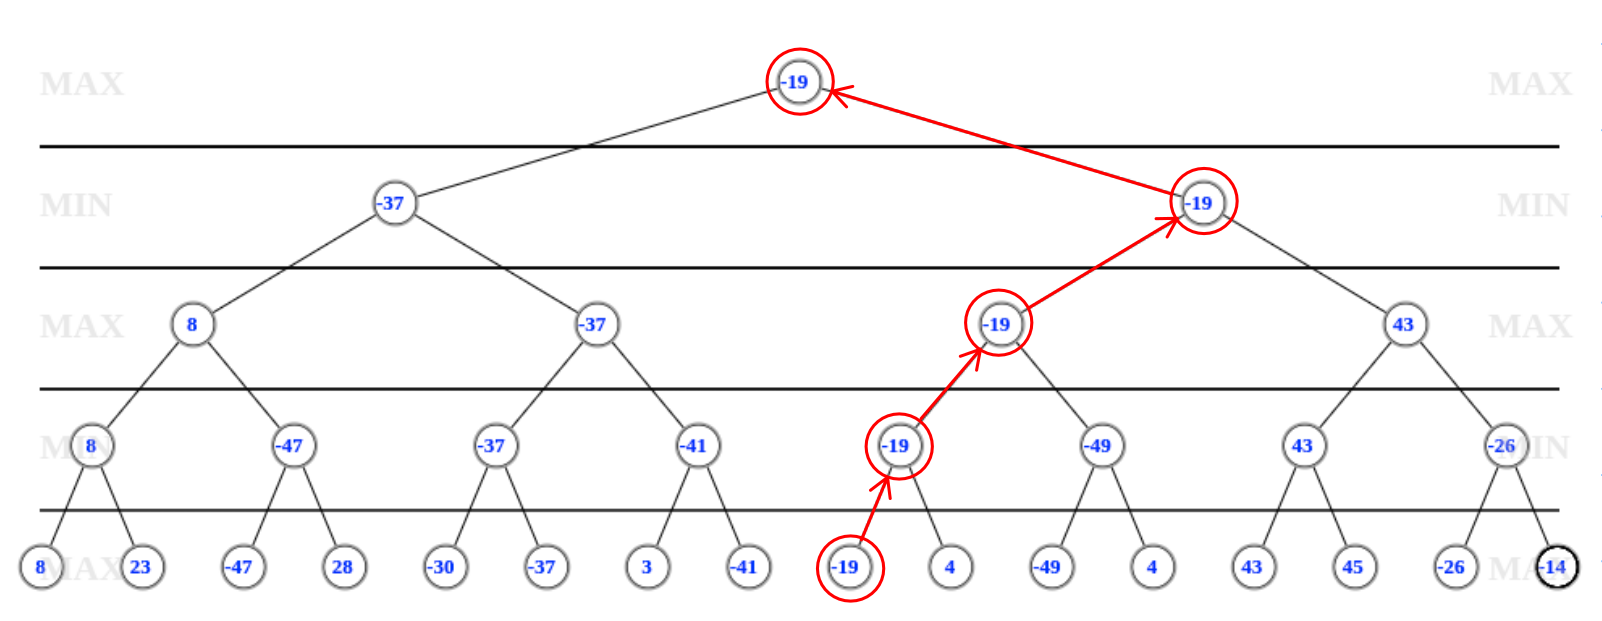
\includegraphics[width=1\textwidth]{images/minimax_example.png}
    \caption{Example de l'exécution de Minimax.}
    \title{fig:Example de l'exécution de Minimax.}
\end{figure}

L’algorithme \texttt{AlphaBeta-pruning} est un algorithme qui a la même
approche que \texttt{Minimax}.\\ Il crée un arbre des coups possibles à une
profondeur donnée et l’explore pour remonter le meilleur score atteignable. La
différence majeure est l’ajout de 2 variables \texttt{Alpha} et \texttt{Beta},
qui mémorisent respectivement le score du meilleur et du pire coup déjà observé
dans la partie explorée de l’arbre.\\ Grâce à ces deux variables, il est
possible de savoir à l’avance s’il est intéressant ou non d’explorer une
branche de l’arbre.\\ S’il n’est pas nécessaire d’explorer une branche (car les
scores obtenus ne sont pas meilleurs que ceux déjà trouvés précédemment), alors
on élague la branche afin d’économiser du temps de calcul.\\
\texttt{AlphaBeta-pruning} renvoie donc le même résultat que \texttt{Minimax}
(avec une profondeur et une heuristique similaire) mais est bien plus efficace
car il n’explore pas systématiquement l’entièreté de l’arbre de jeu.\\ \\ Dans
l'exemple suivant, AlphaBeta remonte les scores des feuilles de la même manière
que Minimax, mais stocke également le meilleur et le pire coup observé dans
alpha et beta. On observe donc l'élagage de certaines branches qui
n'amélioreront en aucun cas les scores alpha et beta. Le résultat est donc le
même, mais l'exploration est plus rapide.

\begin{figure}[h]
    \centering
    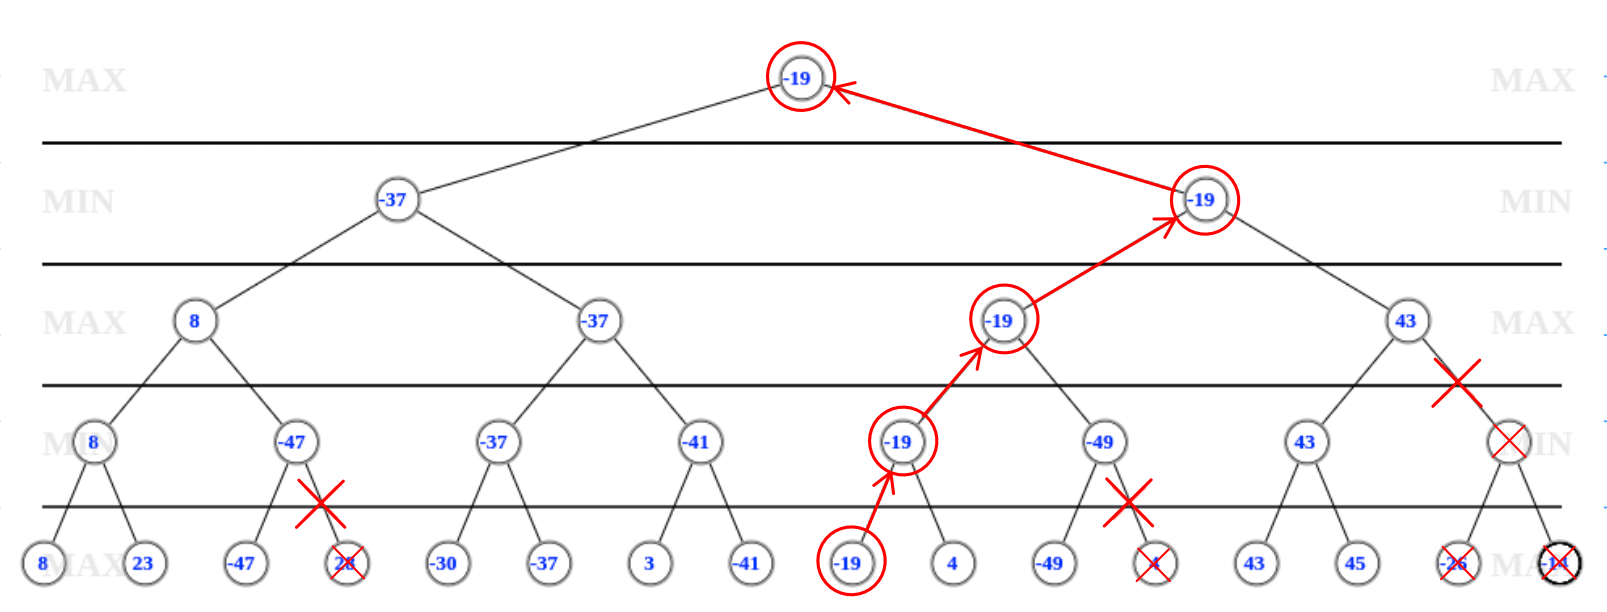
\includegraphics[width=1\textwidth]{images/alphabeta_example.png}
    \caption{Example de l'exécution d'AlphaBeta.}
    \title{fig:Example de l'exécution d'AlphaBeta.}
\end{figure}

Ces deux algorithmes calculent le score des feuilles grâce à nos 4 heuristiques
implémentées, décrites en détails dans le besoin F.51 - Heuristique
d’évaluation de position.\cite{HeuristicPaper}

\newpage

\section{Architecture du projet}

\begin{figure}[h]

    \vspace{3cm}

    \centering
    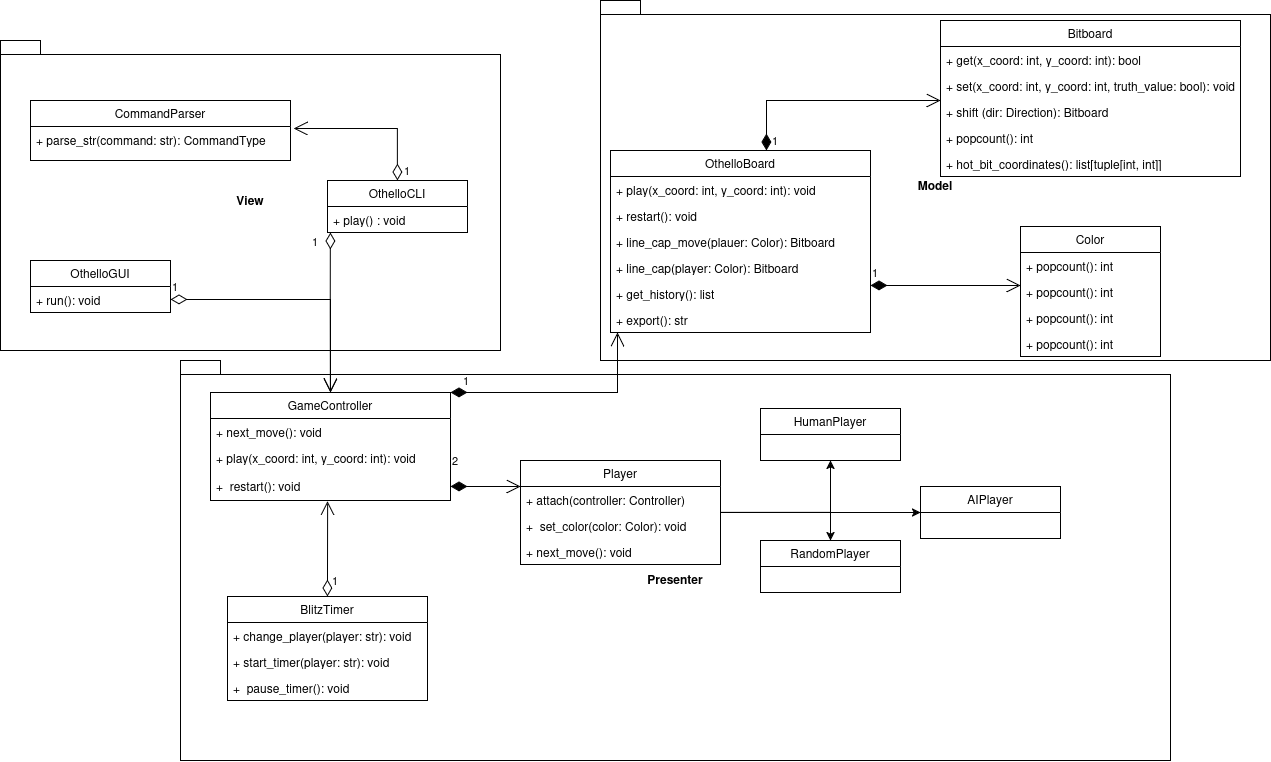
\includegraphics[width=0.9\textwidth]{images/diag_mvp.png}
    \caption{Tâches effectuées pendant la première semaine du projet}
    \title{fig:Diagramme UML de l'architecture du projet}

    \vspace{1cm}

\end{figure}

Nous avons décidé d’adopter une architecture MVC. Ici, nous commencerons par
rappeler brièvement ce que cela implique et comment cela se traduit dans notre
implémentation, avant de détailler le cycle de vie de notre application.\\

\textbf{Le Modèle}\\

Notre application repose sur notre implémentation de \texttt{Bitboard}. En
effet, le jeu d’Othello se prête particulièrement bien à l’utilisation des
\texttt{bitboards} étant donné que l’on peut représenter un état du jeu avec
seulement deux \texttt{bitboards}, un par couleur de joueur.\\ Celle-ci n’est
pas spécifique au jeu d’Othello, mais constitue une implémentation classique de
\texttt{bitboards} tirant parti des particularités du langage \texttt{Python},
telles que l’utilisation par défaut d’entiers de taille arbitraire et la
surcharge d’opérateurs.\\ Pour des raisons de performance, certains attributs
-- comme les masques utilisés -- sont calculés une fois pour toutes, car leur
génération dynamique à chaque instanciation d’un \texttt{bitboard} serait
excessivement coûteuse.\\

Ces \texttt{bitboards} sont directement utilisés par notre modèle,
\texttt{OthelloBoard}, qui gère l’intégralité de l’état d’un plateau de jeu.
Lors de son initialisation, il reçoit une taille issue de l’énumération
\texttt{BoardSize}, qui nous permet également de retrouver un
\texttt{BoardSize} en fonction d’un entier, si celui-ci est une taille de board
valide (6, 8, 10 ou 12).\\ Ce modèle gère ainsi non seulement les deux
\texttt{bitboards} de pions (un pour les noirs, un pour les blancs), mais aussi
l’implémentation des deux algorithmes principaux nécessaires au jeu~:\\
\texttt{line\_cap\_move}~: qui génère un \texttt{bitboard} représentant les
coups possibles pour un joueur donné à partir de l’état actuel du jeu.\\
\texttt{line\_cap}~: qui génère un \texttt{bitboard} des pions capturés à
partir d’un coup (légal) et d’un joueur.\\

Ces algorithmes n’induisent aucune mutation sur le \texttt{bitboard} courant.
Initialement, ils s’appuyaient sur la génération de nombreux \texttt{bitboards}
intermédiaires – ce qui permettait, grâce à la surcharge d’opérateurs,
d’exprimer élégamment les algorithmes.\\ Toutefois, lors d’un
\textit{profiling} visant à réduire la lenteur de l’exploration des arbres de
jeu pour l’IA, nous avons constaté un goulot d’étranglement dû à la création
excessive de ces objets intermédiaires.\\ C’est pourquoi nous avons décidé de
remplacer la boucle de \texttt{line\_cap\_move} par une version déroulée, et
d’optimiser la création ainsi que la copie des \texttt{bitboards}.\\

Pour jouer un coup, c’est-à-dire pour appliquer une mutation sur l’état du
plateau, il faut passer par la fonction \texttt{play()}. Celle-ci reçoit des
coordonnées et, si le coup est possible, le joue pour le joueur courant.\\ En
plus de mettre à jour le plateau, la fonction se charge de changer le joueur
courant, tout en vérifiant si le nouveau joueur courant dispose d’un coup
jouable. Si ce n’est pas le cas, elle enregistre dans l’historique
l’impossibilité pour le nouveau joueur de jouer et rétablit le joueur
initial.\\

Si le joueur initial n’a toujours pas de coup à jouer, le plateau se trouve en
état de « game over ». Même si cela n’implique rien, nous lancions auparavant
une exception, mais celle-ci n’était finalement pas utile puisque vérifiable à
tout moment via \texttt{is\_game\_over()}, ce qui est plus simple que
d’attendre une exception.\\

\newpage

Par ailleurs, \texttt{OthelloBoard} conserve l’historique des coups joués,
permettant, grâce à\\ \texttt{get\_last\_play()}, de retrouver le dernier coup
effectué ou, avec \texttt{pop()}, de retirer ce dernier coup s'il existe. Cette
fonctionnalité a été ajoutée pour faciliter l’exploration des arbres de jeu
dans le cadre de l’implémentation des joueurs IA, afin d’éviter de cloner
l’état avant chaque mutation.\\

Nous obtenons ainsi une modélisation évolutive d’un plateau d’Othello,
respectant les règles de placement de pions, sans pour autant implémenter
d’autres fonctionnalités de base.\\

\textbf{Le Contrôleur (Presenter)}\\

Passons maintenant au contrôleur. \texttt{GameController} se construit à partir
d’un \texttt{OthelloBoard} déjà configuré et de deux joueurs (objets issus
d’une classe dérivée de \texttt{Player}). Il reçoit également les paramètres du
mode blitz : un booléen et un entier indiquant le temps total de jeu si ce mode
est activé.\\ Lors de son instanciation, il crée les deux joueurs en leur
assignant la couleur adéquate (le joueur noir étant créé en premier, le joueur
blanc en second). Il s’enregistre aussi auprès de chaque joueur afin que
ceux-ci puissent appeler la fonction \texttt{play()} du contrôleur lors de leur
action.\\

La méthode \texttt{play()} prend deux coordonnées, \texttt{x\_coord} et
\texttt{y\_coord}, et exécute les étapes suivantes~: - Vérifier que la partie
est toujours en cours en consultant l’attribut \texttt{game\_over} (ce dernier
est mis à \texttt{True} dès que la fin de partie est détectée).\\ - S’assurer
que, dans le mode blitz, le timer du joueur courant n’a pas atteint zéro
(sinon, le joueur perd).\\ - Jouer le coup sur le \texttt{OthelloBoard}.\\ -
Appeler, le cas échéant, un callback \texttt{post\_play\_callback()} (par
exemple, pour actualiser l’affichage dans la CLI).\\ - Changer le joueur
courant pour la gestion du timer de blitz.\\

Cette méthode est invoquée par les vues lorsqu’un joueur humain est en capacité
de jouer.\\

Le contrôlleur se place donc en homme du milieu entre les vues et les modèles.
De fait, nous avons implémentés une architecture Model-View-Presenter.

\textbf{Les Joueurs}\\

La classe \texttt{Player} représente un joueur et lui associe un contrôleur et
une couleur – indispensable pour utiliser des méthodes comme
\texttt{line\_cap\_move()}.\\ Le contrôleur permet quant à lui d’accéder à
\texttt{line\_cap\_move} et de jouer le coup. Pour un joueur humain, la méthode
\texttt{call\_human\_callback()} est appelée lorsqu’il doit jouer.\\ Dans les
faits, cela n’est utilisé que pour le CLI, la GUI se reposant sur
\texttt{current\_player\_is\_human()} du contrôleur pour savoir si le joueur
courant est un humain, méthode appelée à chaque clic sur le board.\\

\textbf{Les Vues}\\

Les vues sont chargées de l’affichage : soit en mode texte dans la CLI, soit
via une fenêtre GTK4 dans la GUI, et elles gèrent également la boucle de jeu.
\\ Bien que le contrôleur détermine l’état de la partie (par exemple, en
bloquant l’action en cas de « game over »), ce sont les vues qui envoient les
actions. La principale différence réside dans la gestion des entrées : en CLI,
l’utilisateur est sollicité de manière bloquante, tandis qu’en GUI, c’est le
clic de l’utilisateur qui déclenche l’action.\\ À chaque clic, la vue vérifie
si le contrôleur attend un coup de la part d’un joueur humain et, si c’est le
cas, le joue. \\ De plus, dans le cas de la GUI, la boucle de jeu est gérée par
GTK via des callbacks, contrairement à la CLI où le contrôleur appelle
directement la méthode \texttt{next\_move()} dans sa boucle de jeu.\\

\textbf{Cycle de Vie de l’Application}\\

Le point d’entrée de l’application est \texttt{\_\_main\_\_.py}. Celui-ci
commence par récupérer un objet de configuration (\texttt{Config}) via
\texttt{argparse}.\\ Si un nom de fichier est fourni, il tente de charger cet
état dans un \texttt{OthelloBoard}, sinon, il initialise un
\texttt{OthelloBoard} avec la taille indiquée en argument ou par défaut.\\
Ensuite, les deux joueurs (noir et blanc) sont créés, en tenant compte de la
présence ou non d’un joueur IA.\\ Le contrôleur est ensuite initialisé en
fonction du mode blitz, puis transmis à la vue adéquate, laquelle lance la
boucle de jeu (pour la CLI) ou le démarrage de GTK (pour la GUI).\\

\newpage

\section{Performances et limitations}

\textbf{Mesure des performances et problèmes initiaux}\\

Les performances du code, ainsi que les temps de calcul des intelligences
artificielles (IA) utilisant différentes heuristiques, ont été évalués à l’aide
du module \texttt{time} de Python.\\ Cependant, lors des tests avec des
profondeurs de recherche élevées (6, 7 et 8), des limitations significatives
sont apparues, entraînant des temps d’exécution prohibitifs. Ces contraintes
ont motivé une analyse approfondie des méthodes employées, en particulier
celles reposant sur les \texttt{bitboards}.\\

\begin{figure}[h]

    \centering
    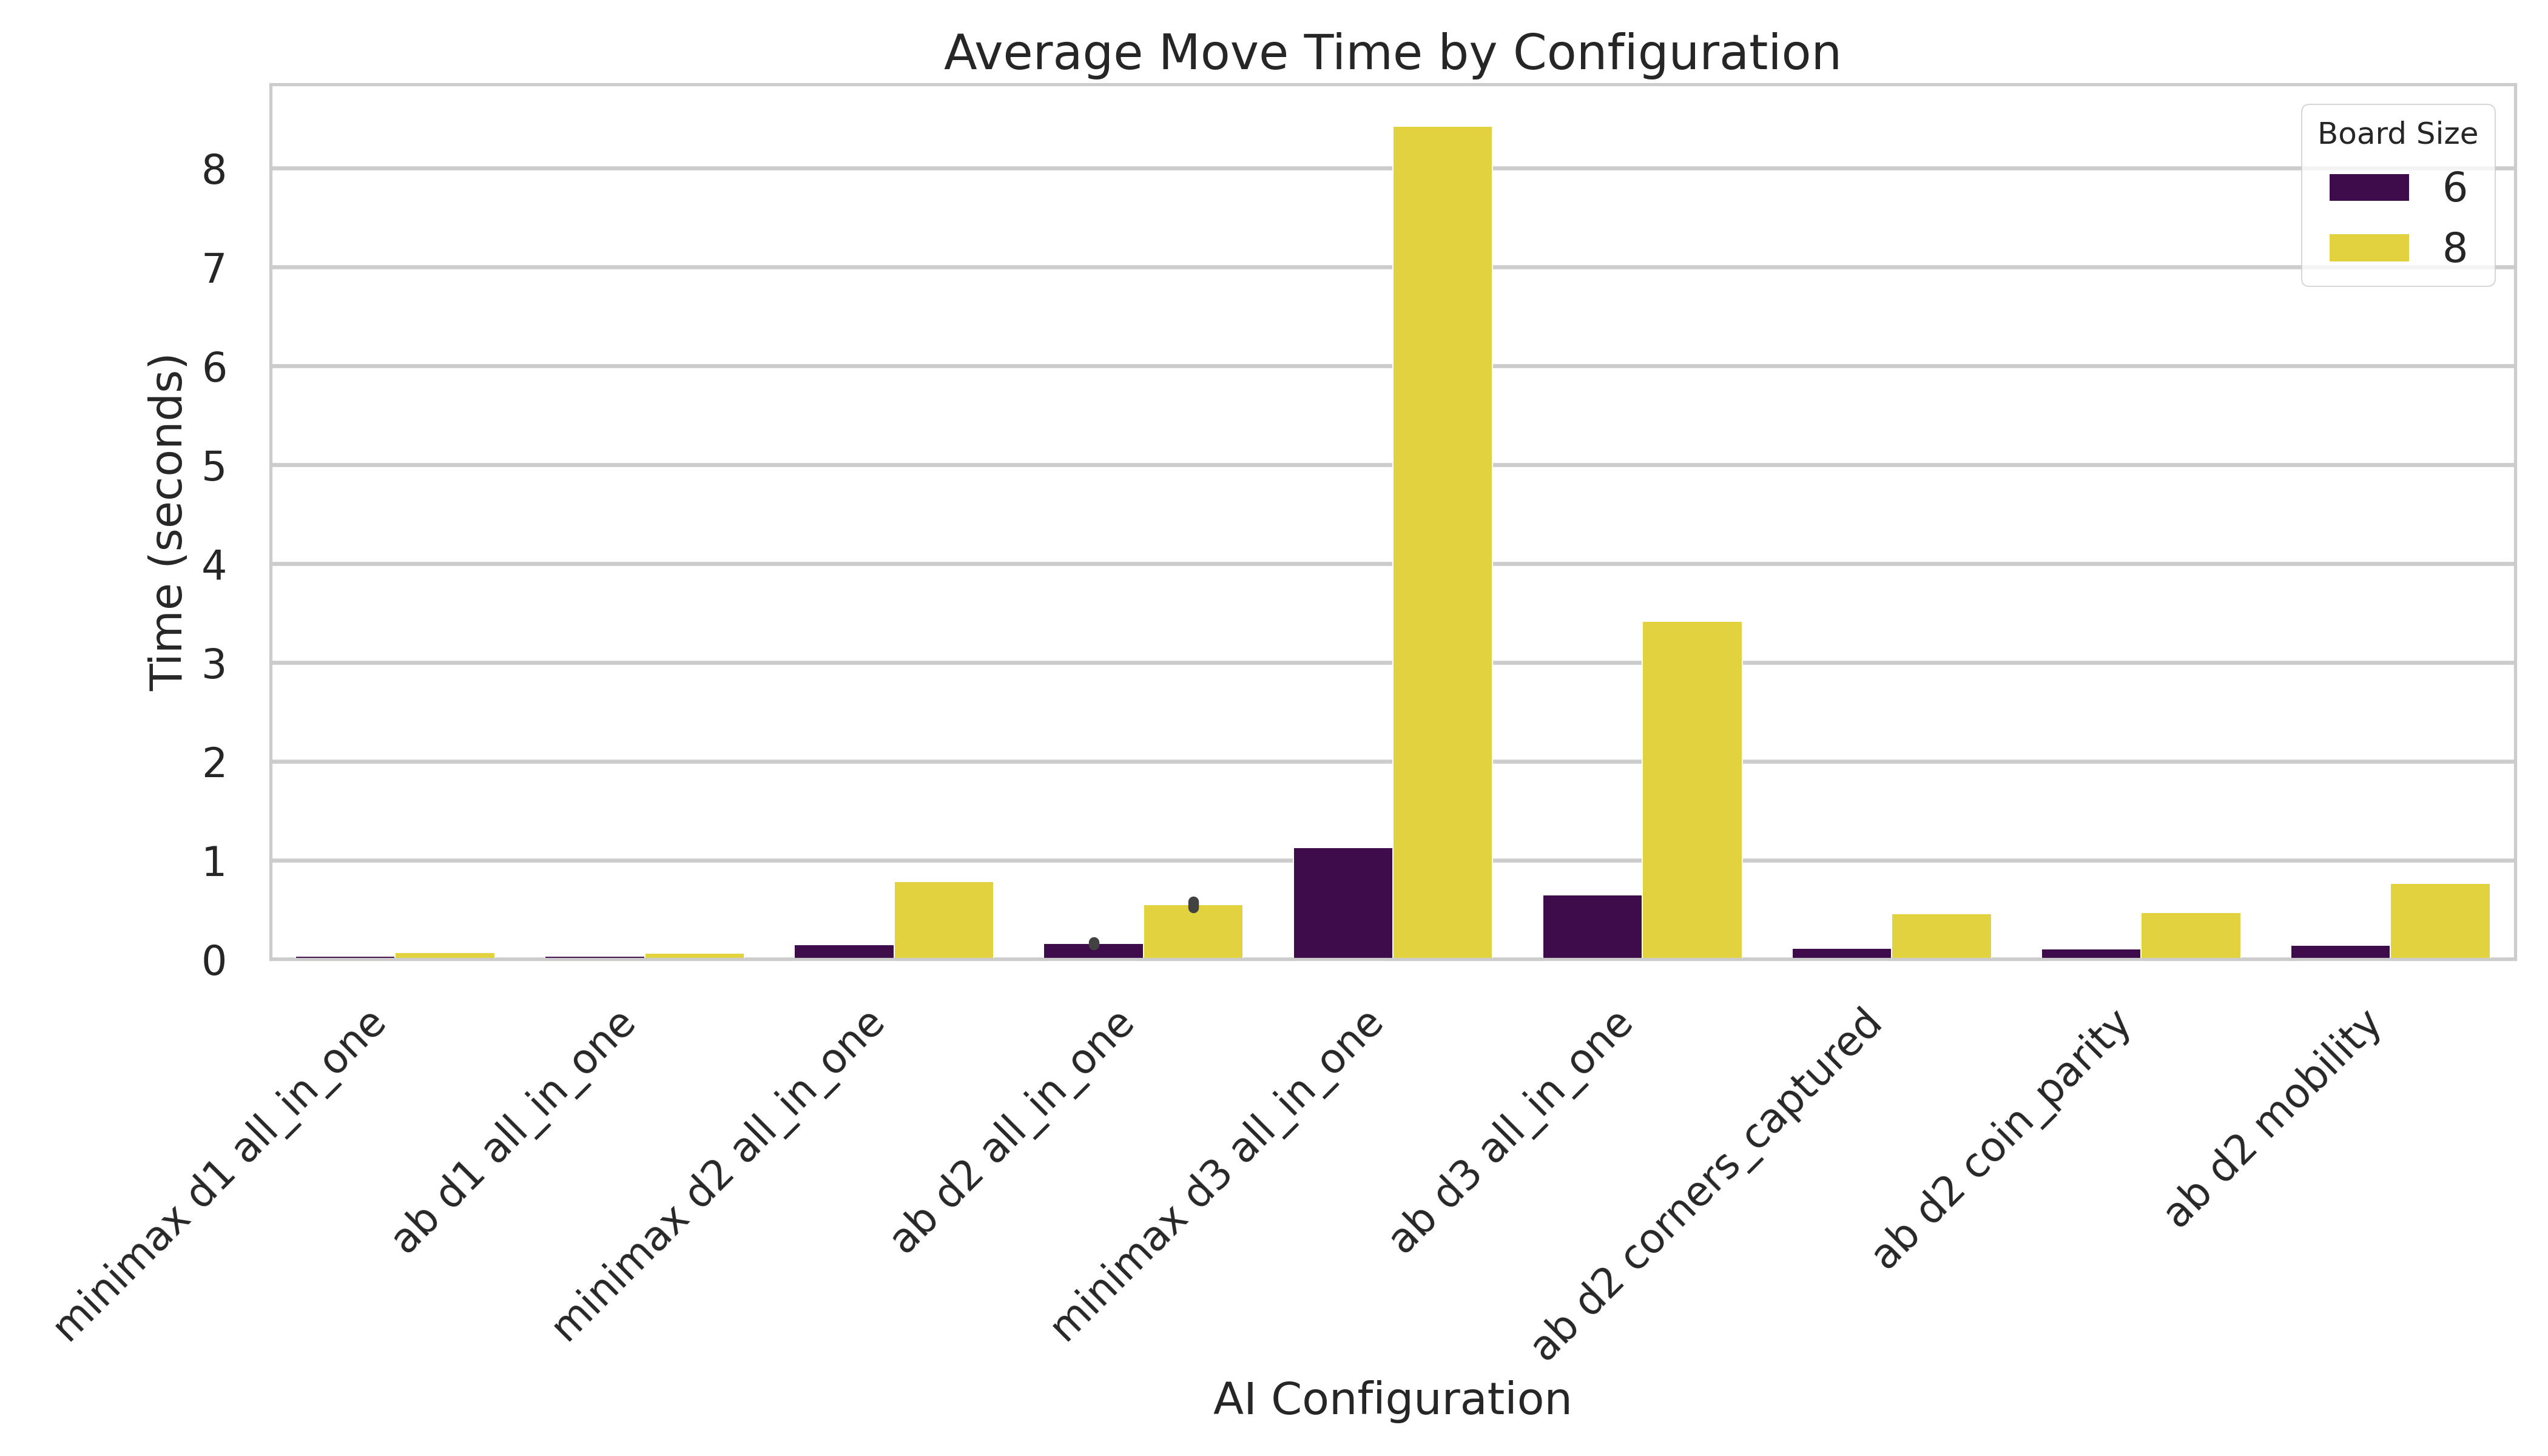
\includegraphics[width=0.9\textwidth]{images/time_comparison_config.png}
    \caption{Temps de calcul par tour pour une configuration donnée.}
    \title{fig:time_comparison_config.png}

\end{figure}

\textbf{Optimisations apportées}\\

Un premier diagnostic, réalisé à l’aide de PyCharm et du profilé intégré
(\texttt{cProfiler}), a révélé des inefficacités critiques dans la manipulation
des \texttt{bitboards}. Parmi les problèmes identifiés :\\ - Une vérification
bit-à-bit systématique lors de chaque opération sur le plateau, même dans les
cas où aucun mouvement n’était joué.\\ - Une surcharge inutile dans la méthode
\texttt{get(cls, size) -> int}, pénalisant les performances globales.\\ Après
révision de ces méthodes, une optimisation majeure a été implémentée, réduisant
drastiquement le temps de calcul. La \textbf{figure 9} illustre l’amélioration
obtenue, comparant le coût temporel d’un tour avant et après cette
modification.\\

\newpage

\textbf{Comparaison des algorithmes : Minimax vs Alpha-Beta}\\

Pour affiner nos résultats, nous avons comparé les performances des algorithmes
\texttt{Minimax} et \texttt{Alpha-Beta}. Comme attendu, ce dernier s’est avéré
significativement plus rapide grâce à son mécanisme d’élagage. La
\textbf{Figure 2} présente cette comparaison, confirmant que
\texttt{Alpha-Beta} est mieux adapté à nos besoins.\\

\begin{figure}[h]
    \centering
    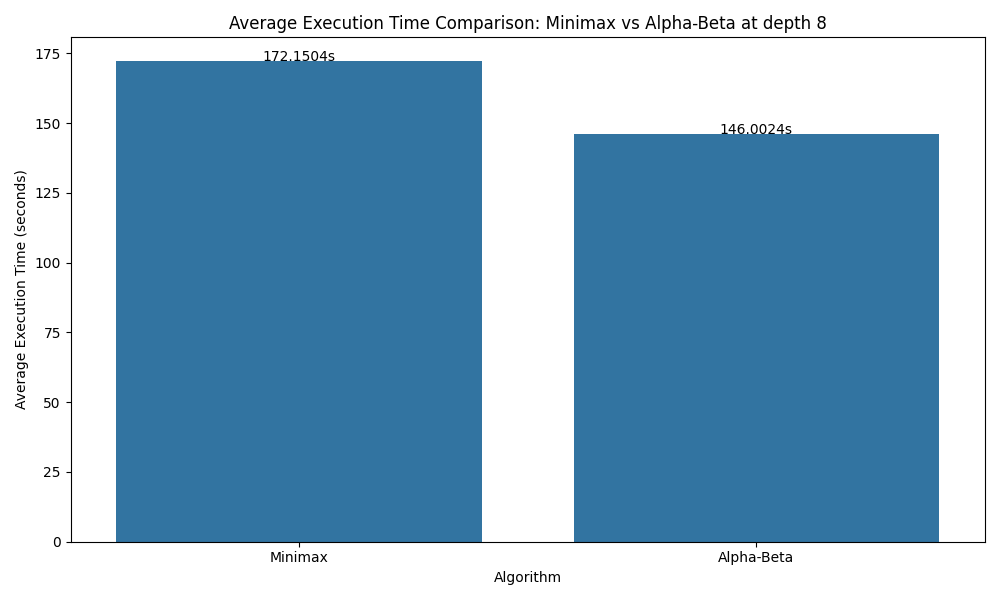
\includegraphics[width=0.9\textwidth]{images/algorithm_time_comparison.png}
    \caption{TFigure 2: Minimax vs Alpha-Beta à profondeur 8.}
    \title{fig:algoritm_time_comparison.png}
\end{figure}

\noindent Suite à ces observations, \texttt{Alpha-Beta} a été retenue pour toutes
les expériences suivantes.\\

\newpage

\textbf{Évaluation des heuristiques et biais potentiels}\\

Enfin, nous avons mesuré l’impact des différentes heuristiques en fonction de
la profondeur de recherche.

\begin{figure}[h]
    \centering
    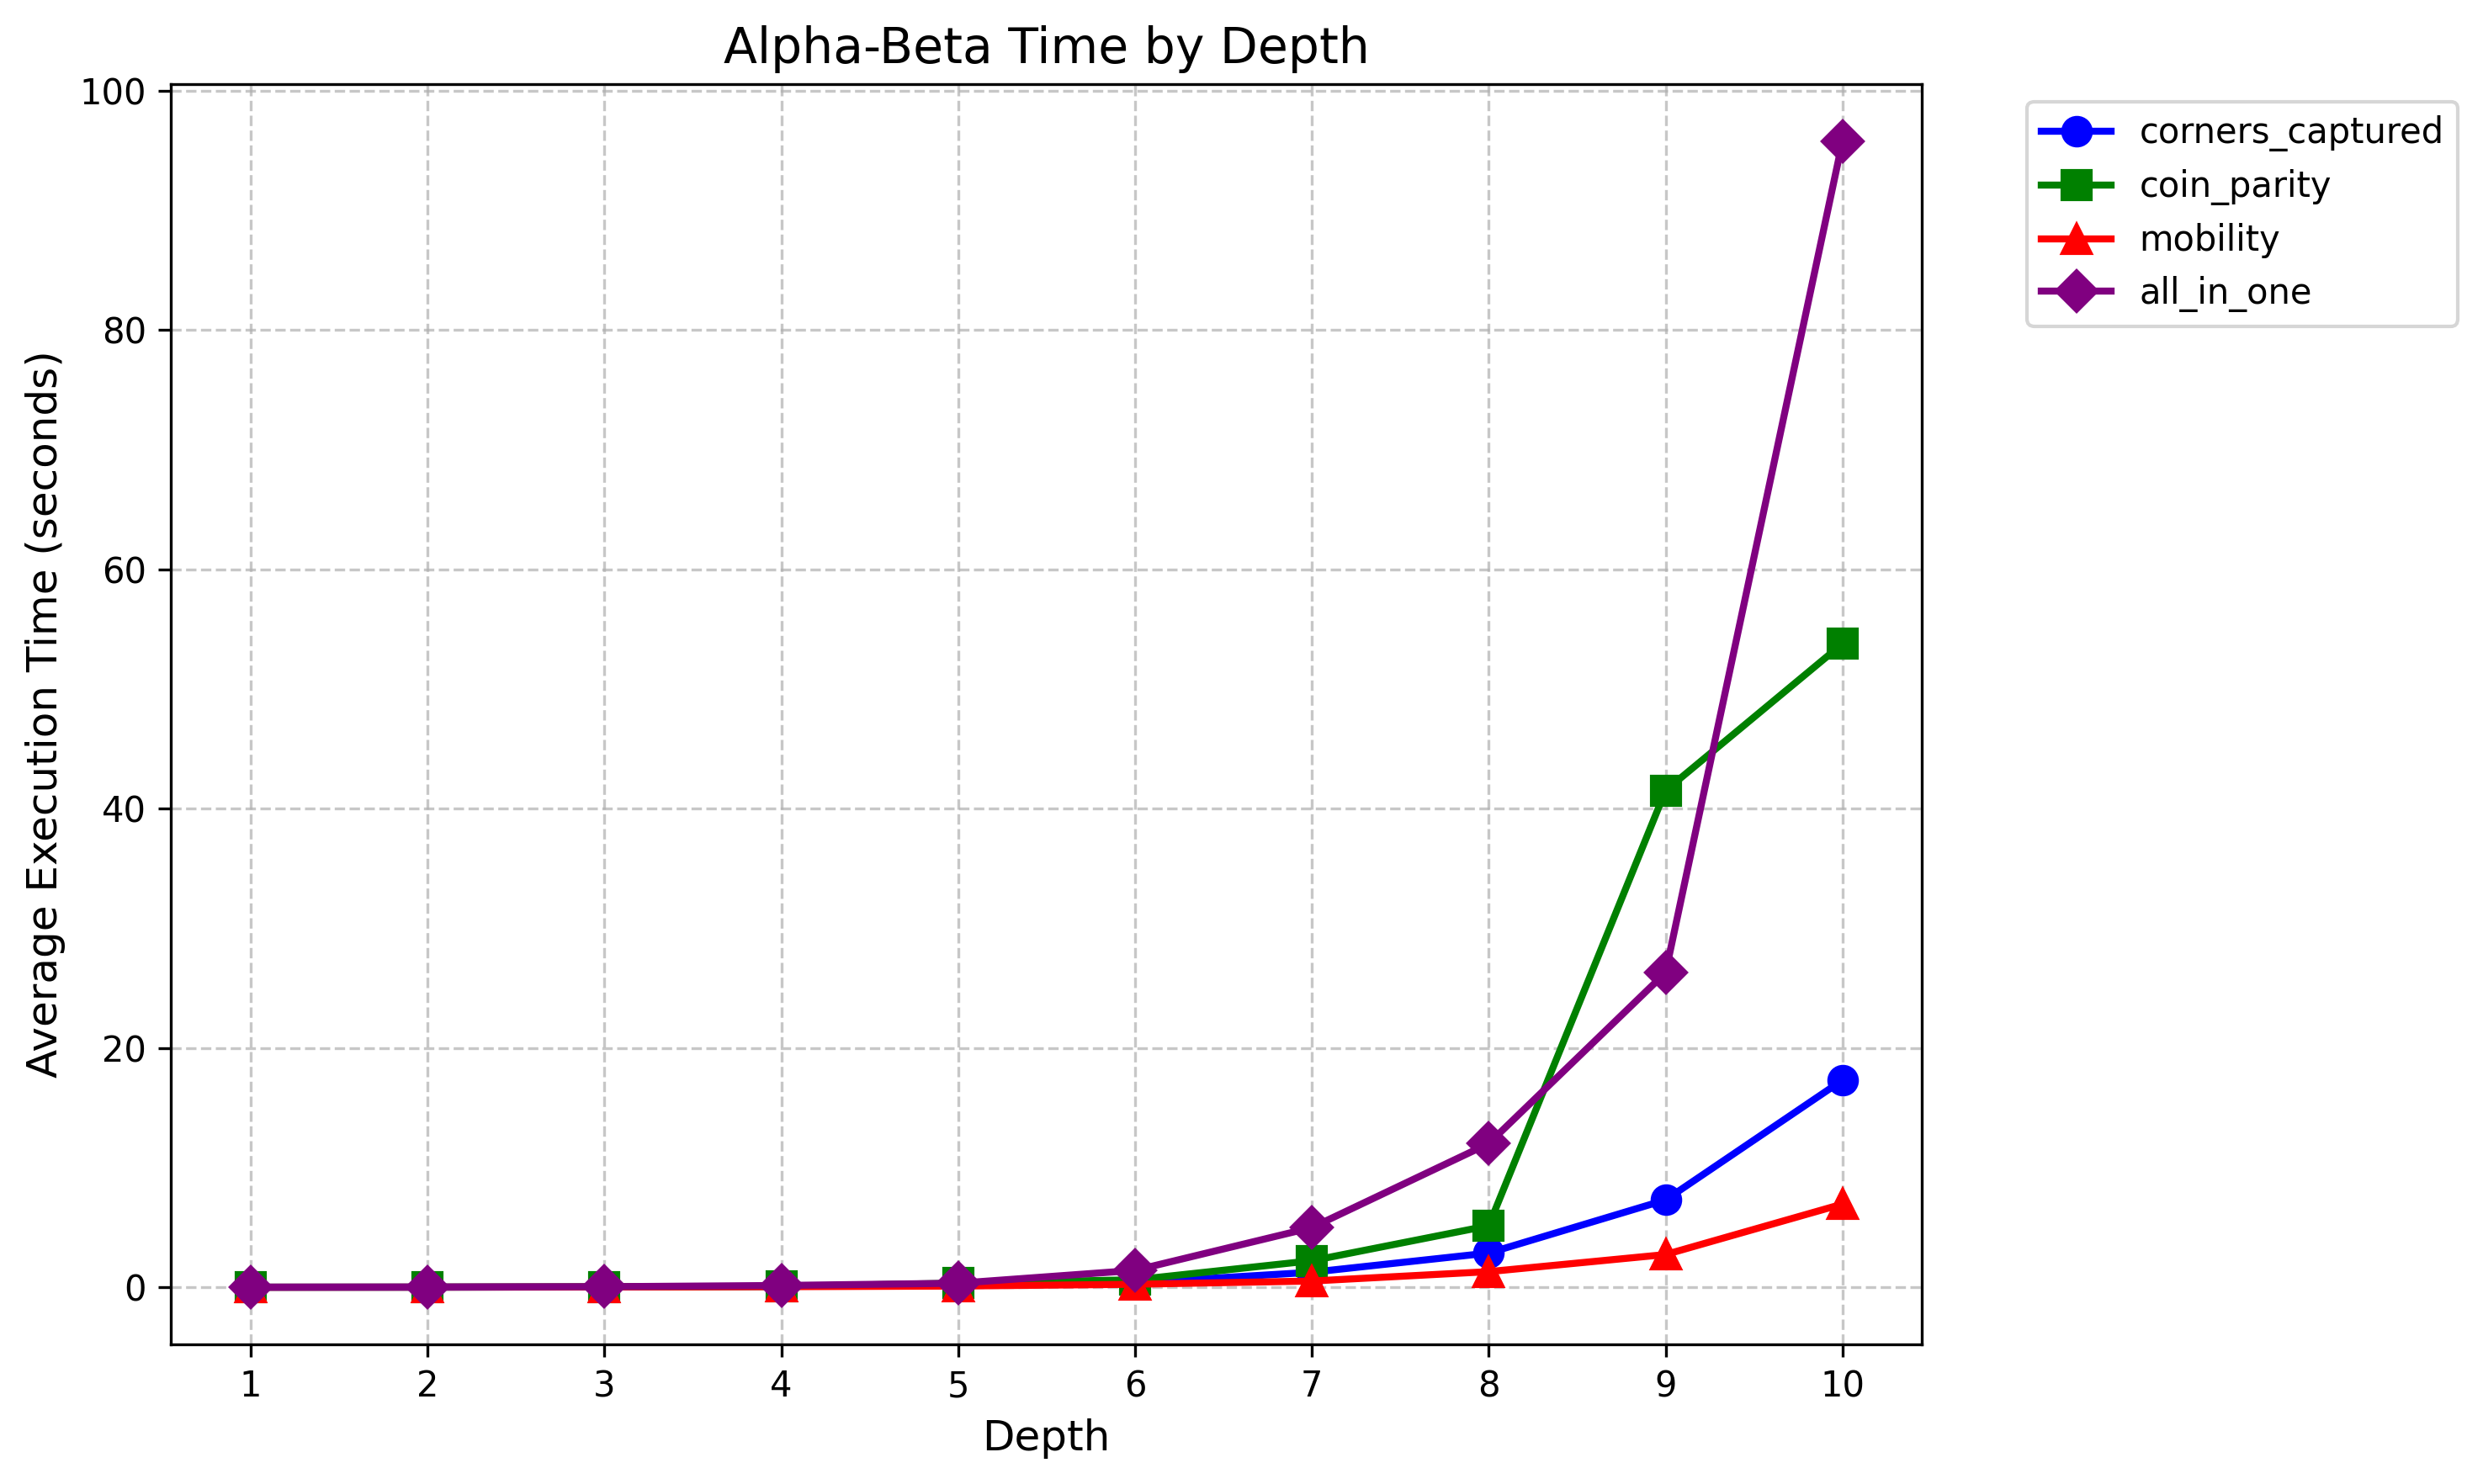
\includegraphics[width=0.9\textwidth]{images/alpha_beta_time_by_depth.png}
    \caption{TFigure 2: Minimax vs Alpha-Beta à profondeur 8.}
    \title{fig:alpha_beta_time_by_depth.png}
\end{figure}

\FloatBarrier

Par ailleurs, une question cruciale a été investiguée : Othello présente-t-il
un biais en fonction du côté (noir/blanc) avec lequel on débute ?\\ Pour y
répondre, des tests ont été menés avec \texttt{coin\_parity} à une profondeur
de 6, permettant de collecter des données statistiques sur les taux de
victoire. En effet, environ 52\% du temps le deuxième joueur gagne, c’est dû au
fait qu'il posera la dernière pièce en cas d’un tableau rempli.\\

\textbf{Limitations:}\\

Nous voyons avec nos résultats qu'à partir d’une profondeur 7, le jeu se
ralentit considérablement, puis à une profondeur 9, le temps par coup est
d'environ 40 secondes, ce qui est injouable.\\ De plus, en Python, les entiers
n’ont pas de limite de grandeur. Nous avons mis la limite à un tableau de 10x10
avant qu'une machine de configuration moyenne commence à attendre sa limite.\\

\newpage

\section{Critiques et perspectives}
L’étape préliminaire de familiarisation avec le sujet s’est globalement
déroulée sans encombre. Seule une mauvaise répartition initiale des besoins a
freiné notre progression, nous faisant perdre environ deux semaines.\\ Après
redistribution des besoins, notre efficacité s’est nettement améliorée~: le
projet prenait davantage de sens, ce qui rendait le travail plus motivant et
agréable.\\

Le cahier des charges n’a pas été respecté à 100~\%~: certains besoins ont été
partiellement ou totalement laissés de côté, nous ne pouvons donc pas dire qu’à
l’arrivée de la fin du projet, le logiciel répond à toutes les attentes.\\

Cependant, le logiciel livré à la date de rendu reste complet. Les modes de jeu
et les options implémentées sont pertinents et pleinement fonctionnels.\\ Les
fonctionnalités négligées n’étaient pas essentielles au bon fonctionnement de
l’application~; elles correspondaient plutôt à des améliorations ou des
extensions futures. C’est pourquoi nous estimons que livrer le projet dans son
état actuel est acceptable pour une première version.\\ Nous considérons avoir
abouti à une première version solide et cohérente.\\

Au départ, notre équipe était composée de cinq membres. L’un d’entre nous a
participé aux réflexions initiales, mais son implication a rapidement diminué,
tant dans les discussions que dans l’implémentation du projet.\\ Son manque de
contribution a entraîné quelques ralentissements, notamment au lancement du
projet, mais nous avons su nous adapter et redistribuer les tâches
efficacement.\\ L’un des autres défis majeurs a été la coordination de nos
emplois du temps.\\ Entre les différentes spécialisations et obligations de
chacun, trouver des créneaux communs pour travailler s’est révélé compliqué.\\

La majorité des besoins définis en amont ont été traités. Le peu de besoins non
terminés ont néanmoins été étudiés, et parfois partiellement implémentés.\\
Mais à l’approche de la date de rendu, nous avons préféré abandonner leur
implémentation pour nous concentrer sur un code propre, testé, avec le moins de
bugs possible plutôt que d’ajouter des fonctionnalités non finalisées.\\

Concernant la gestion des erreurs, nous avons veillé à ce que les entrées
utilisateur soient correctement prises en compte.\\ Selon que le logiciel ait
été lancé ou non, une erreur d’entrée ne fait que redemander une entrée à
l’utilisateur, et affiche une aide.\\ La plupart des erreurs, qu’elles soient
liées aux entrées ou aux valeurs dans d’autres fonctions, renvoient un message
clair et un traçage de l’erreur.\\ Cette gestion est principalement assurée
dans les fonctions appelées, avec parfois une vérification supplémentaire dans
les fonctions appelantes.\\

En ce qui concerne la maintenance et les perspectives d’évolution de notre
logiciel, plusieurs axes d’amélioration sont envisageables.\\ Dans un premier
temps, il serait pertinent de compléter l’implémentation des besoins
initialement prévus.\\ Nous pourrions également enrichir notre intelligence
artificielle et notre interface graphique, notamment en ajoutant des
heuristiques plus complexes, une recherche de type Monte Carlo, ainsi que des
menus et la possibilité de modifier la configuration sur notre GUI.\\

À plus long terme, nous pourrions envisager une interface web, avec un portage sur plusieurs plateformes, et potentiellement rajouter un mode de jeu en ligne, avec un système de rang ou de points.\\
Pour cela, la documentation présente dans ce rapport, ainsi que des indications plus détaillées à destination de futurs développeurs, seront des ressources nécessaires en vue d’une future phase de développement.\\

Nous restons ouverts aux retours de nos pairs et de nos enseignants, qui seront
pris en compte avec attention dans l’éventualité d’une poursuite du projet.
Toute critique constructive, qu’elle soit positive ou négative, est la
bienvenue.\\

Même si ce projet s’inscrit dans un cadre scolaire et qu’aucune suite n’est
actuellement prévue, la base de code reste la nôtre.\\ Il n’est donc pas exclu
que nous décidions de le faire évoluer de notre côté.\\

\newpage

\appendix
\section{Liste des besoins étendus}

\vspace{1cm}

\noindent
\setlength{\arrayrulewidth}{1.5pt}
\renewcommand{\arraystretch}{1.5}
\arrayrulecolor{RoyalBlue}
\begin{tabularx}{\textwidth}{|X|}
    \hline
    \textbf{F.1 Langage de programmation}          \\
    \hline
    Besoin non fonctionnel                         \\
    \hline
    Terminé le 06/02                               \\
    Par Lucas                                      \\
    \hline
    Développer le logiciel en langage Python 3.7+. \\
    \hline
\end{tabularx}

\vspace{1cm}

\noindent
\setlength{\arrayrulewidth}{1.5pt}
\renewcommand{\arraystretch}{1.5}
\arrayrulecolor{RoyalBlue}
\begin{tabularx}{\textwidth}{|X|}
    \hline
    \textbf{F.2 - Style de codage}                                                          \\
    \hline
    Besoin non fonctionnel                                                                  \\
    \hline
    Terminé le 04/02                                                                        \\
    Par Lucas                                                                               \\
    \hline
    Le code du programme suit le coding style du PEP8.                                      \\
    L’utilisation de pre-commit hooks permet de s’assurer du respect de ce style de codage. \\
    \hline
\end{tabularx}

\vspace{1cm}

\noindent
\setlength{\arrayrulewidth}{1.5pt}
\renewcommand{\arraystretch}{1.5}
\arrayrulecolor{RoyalBlue}
\begin{tabularx}{\textwidth}{|X|}
    \hline
    \textbf{F.3 - Langue par défaut du code}                                                                            \\
    \hline
    Besoin non fonctionnel                                                                                              \\
    \hline
    Terminé le 02/02                                                                                                    \\
    Par Matis, Rémy, Lucas, Gabriel                                                                                     \\
    \hline
    Le code, la documentation ainsi que les fichiers annexes sont écrits et commentés intégralement en langue anglaise. \\
    \hline
\end{tabularx}

\vspace{1cm}

\noindent
\setlength{\arrayrulewidth}{1.5pt}
\renewcommand{\arraystretch}{1.5}
\arrayrulecolor{RoyalBlue}
\begin{tabularx}{\textwidth}{|X|}
    \hline
    \textbf{F.4 - Système cible
    }                                                                                               \\
    \hline
    Besoin non fonctionnel                                                                          \\
    \hline
    Terminé le 06/02                                                                                \\
    Par Lucas Zammit                                                                                \\
    \hline
    Développement du logiciel sous une distribution Linux.                                          \\
    L’intégration de Python rend compliqué voir impossible l’installation de modules
    python sur l’environnement par défaut.                                                          \\
    Sur les systèmes Debian récents, il est donc nécessaire de passer par un environnement virtuel. \\
    \arrayrulecolor{MediumAquamarine}\hline
    \arrayrulecolor{RoyalBlue}
    Tester sous une distribution Linux Debian, et une distribution Ubuntu.                          \\
    \hline
\end{tabularx}

\vspace{1cm}

\noindent
\setlength{\arrayrulewidth}{1.5pt}
\renewcommand{\arraystretch}{1.5}
\arrayrulecolor{RoyalBlue}
\begin{tabularx}{\textwidth}{|X|}
    \hline
    \textbf{F.5 - Documentation}                                                                                                                                                                                                                                           \\
    \hline
    Besoin non fonctionnel                                                                                                                                                                                                                                                 \\
    \hline
    Terminé le 19/03                                                                                                                                                                                                                                                       \\
    Par Matis, Rémy, Lucas, Gabriel                                                                                                                                                                                                                                        \\
    \hline
    Une documentation Sphinx automatisée permet de rendre compte des différentes fonctions, leurs attributs et leur utilité pour chaque module.                                                                                                                            \\
    Le code est documenté à l’aide de docstrings et commentaires.                                                                                                                                                                                                          \\
    Un manuel utilisateur, ainsi qu’un manuel utilisateur pour les développeurs sont disponibles. Ils proposent des explications pour l’installation et l’utilisation du logiciel d’un point de vue utilisateur, et en proposant plus de précisions pour les développeurs. \\
    Une option d’aide est présente en dehors d’une partie, afin d’indiquer à l’utilisateur comment lancer une partie et quelles options sont à sa disposition.                                                                                                             \\
    En cours de partie, une option d’aide et une présentation des règles du jeu est également disponible.                                                                                                                                                                  \\
    \hline
\end{tabularx}

\vspace{1cm}

\noindent
\setlength{\arrayrulewidth}{1.5pt}
\renewcommand{\arraystretch}{1.5}
\arrayrulecolor{RoyalBlue}
\begin{tabularx}{\textwidth}{|X|}
    \hline
    \textbf{F.6 - Tests}                                                                                                                                                                     \\
    \hline
    Besoin non fonctionnel                                                                                                                                                                   \\
    \hline
    Terminé le 07/03                                                                                                                                                                         \\
    Par Matis, Rémy, Lucas, Gabriel                                                                                                                                                          \\
    \hline
    Les fonctionnalités du logiciel sont testées automatiquement. Il est possible de les lancer avec la commande \texttt{pytest} à la racine du projet ou dans le dossier \texttt{othello/}. \\
    L’automatisation des tests est intégrée à la pipeline CI gitlab.                                                                                                                         \\
    Ces tests couvrent au minimum 80\% du code écrit.                                                                                                                                        \\
    \hline
\end{tabularx}

\vspace{1cm}
\noindent
\setlength{\arrayrulewidth}{1.5pt}
\renewcommand{\arraystretch}{1.5}
\arrayrulecolor{RoyalBlue}
\begin{tabularx}{\textwidth}{|X|}
    \hline
    \textbf{F.7 - Bugs}                                                                                                                                                                                                              \\
    \hline
    Besoin non fonctionnel                                                                                                                                                                                                           \\
    \hline
    Terminé le 08/04                                                                                                                                                                                                                 \\
    Par Matis, Rémy, Lucas, Gabriel                                                                                                                                                                                                  \\
    \hline
    L’implémentation des fonctionnalités du logiciel seront robustes - dans la mesure du possible - aux éventuelles mauvaises entrées de l’utilisateur, ou à d’autres cas amenant à des bugs.                                        \\
    \arrayrulecolor{MediumAquamarine}\hline
    \arrayrulecolor{RoyalBlue}
    Afin de pallier d'éventuels bugs menant à un crash du logiciel, les fonctionnalités sont testées le plus possible, et les erreurs d’entrées ou d’arguments sont traitées et renvoient une erreur compréhensible à l’utilisateur. \\
    \hline
\end{tabularx}

\vspace{1cm}

\noindent
\setlength{\arrayrulewidth}{1.5pt}
\renewcommand{\arraystretch}{1.5}
\arrayrulecolor{RoyalBlue}
\begin{tabularx}{\textwidth}{|X|}
    \hline
    \textbf{F.8 - Performances}                                                                                                                  \\
    \hline
    Besoin non fonctionnel                                                                                                                       \\
    \hline
    Terminé le 07/04                                                                                                                             \\
    Par Matis                                                                                                                                    \\
    \hline
    Ajout de l’option \texttt{-}\texttt{-benchmark} pour mesurer les performances des IA avec un choix d’heuristique ainsi que de mode.          \\
    \arrayrulecolor{MediumAquamarine}\hline
    \arrayrulecolor{RoyalBlue}
    Afin de faire des tests variés, nous avons changé la configuration de base pour y accueillir des options d’IA des deux cotés, noir et blanc. \\
    Placés dans le répertoire benchmark, il suffit de lancer \texttt{run\_experiments.py}.                                                       \\
    \hline
\end{tabularx}

\vspace{1cm}

\noindent
\setlength{\arrayrulewidth}{1.5pt}
\renewcommand{\arraystretch}{1.5}
\arrayrulecolor{RoyalBlue}
\begin{tabularx}{\textwidth}{|X|}
    \hline
    \textbf{F.9 - Build-system}                                                                                                                                \\
    \hline
    Besoin non fonctionnel                                                                                                                                     \\
    \hline
    Terminé le 04/02                                                                                                                                           \\
    Par Rémy                                                                                                                                                   \\
    \hline
    Le build-system est basé sur \texttt{pyproject.toml} et \texttt{septuptools}.                                                                              \\
    Les métadonnées du projet sont définies (nom, version, auteurs…) dans le \texttt{pyproject.toml}, ainsi que les dépendances et scripts associés au projet. \\
    De plus, les stratégies de test et de coverage sont également définies dans le \texttt{pyproject.toml}.                                                    \\
    \hline
\end{tabularx}

\vspace{1cm}

\noindent
\setlength{\arrayrulewidth}{1.5pt}
\renewcommand{\arraystretch}{1.5}
\arrayrulecolor{RoyalBlue}
\begin{tabularx}{\textwidth}{|X|}
    \hline
    \textbf{F.10 - Framework de tests}                            \\
    \hline
    Besoin non fonctionnel                                        \\
    \hline
    Terminé le 04/02                                              \\
    Par Matis et Lucas                                            \\
    \hline
    Mise en place de la pipeline CI/CD dans git.
    Avant chaque commit, les tests seront lancés par la pipeline. \\
    Utilisation du framework de tests Pytest et de Coverage.      \\
    \hline
\end{tabularx}

\vspace{1cm}

\noindent
\setlength{\arrayrulewidth}{1.5pt}
\renewcommand{\arraystretch}{1.5}
\arrayrulecolor{CornflowerBlue}
\begin{tabularx}{\textwidth}{|X|}
    \hline
    \textbf{F.11 - Gestion des options}                                                                                                                                             \\
    \hline
    Besoin fonctionnel                                                                                                                                                              \\
    \hline
    Terminé le 18/02                                                                                                                                                                \\
    Par Gabriel                                                                                                                                                                     \\
    \hline
    Les options en lignes de commandes pour le lancement d’une partie sont gérées par le module argparse qui construit un objet contenant les arguments donnés par l’utilisateur.   \\
    Les arguments passés au programme prennent systématiquement la priorité sur les
    paramètres définis dans le fichier de configuration othello, qui lui-même aura la priorité
    sur les paramètres par défaut.                                                                                                                                                  \\

    Les fonctions principales implémentées sont les suivantes :                                                                                                                     \\
    \texttt{create\_parser() -> ArgumentParser}, qui initialise et configure le
    parseur d’arguments ;                                                                                                                                                           \\ \texttt{parse\_args() -> tuple[str, dict[str, Any]]},
    qui parse les arguments, et gère les potentielles erreurs d’entrée : si
    l’utilisateur a entré de mauvais arguments, ou une option non reconnue ;                                                                                                        \\ et
    \texttt{parse\_error(parser: ArgumentParser, message: str) -> None}, qui
    affiche des messages d’erreurs dans la console, en utilisant la sortie d’erreur
    standard.                                                                                                                                                                       \\

    \arrayrulecolor{MediumAquamarine}\hline
    \arrayrulecolor{CornflowerBlue}
    Validation du parseur avec une configuration par défaut, avec un fichier de configuration, et avec les différentes options disponibles.                                         \\
    Validation de la gestion d’erreurs avec des configurations invalides : option non existante ou dont la valeur donnée n’est pas acceptable, incompatibilité des modes de jeu.    \\
    \arrayrulecolor{MediumAquamarine}\hline
    \arrayrulecolor{CornflowerBlue}
    Nécessite la définition d’un fichier de configuration (F.40), afin de connaître toutes les options que le parseur doit proposer à l’utilisateur pour le lancement d’une partie. \\
    Nécessaire pour lancer le jeu (F.15), ainsi que les différents modes de jeu et l’affichage de messages à l’utilisateur (besoins F.16 à F.24).                                   \\
    \hline
\end{tabularx}

\vspace{1cm}

\noindent
\setlength{\arrayrulewidth}{1.5pt}
\renewcommand{\arraystretch}{1.5}
\arrayrulecolor{RoyalBlue}
\begin{tabularx}{\textwidth}{|X|}
    \hline
    \textbf{F.12 - Bibliothèque graphique}                            \\
    \hline
    Besoin non fonctionnel                                            \\
    \hline
    Terminé le 27/02                                                  \\
    Par Lucas                                                         \\
    \hline
    Utilisation de la bibliothèque graphique PyGObject.               \\
    Utilisation de la version 4.0 de Gtk.                             \\
    \hline
    \arrayrulecolor{RoyalBlue}
    Nécessaire pour l’implémentation de l’interface graphique (F.26). \\
    \hline
\end{tabularx}

\vspace{1cm}

\noindent
\setlength{\arrayrulewidth}{1.5pt}
\renewcommand{\arraystretch}{1.5}
\arrayrulecolor{RoyalBlue}
\begin{tabularx}{\textwidth}{|X|}
    \hline
    \textbf{F.14 - Nom du programme}                                                                                                                 \\
    \hline
    Besoin non fonctionnel                                                                                                                           \\
    \hline
    Terminé le 09/02                                                                                                                                 \\
    Par Lucas                                                                                                                                        \\
    \hline
    Le logiciel pourra être lancé avec l’exécutable \texttt{othello}.                                                                                \\
    Taper \texttt{othello} dans l’invite de commande permet de lancer une partie en mode normal, joueur contre joueur, sur un plateau de huit cases. \\
    Il sera nécessaire de lancer le programme depuis un environnement virtuel.                                                                       \\
    \hline
\end{tabularx}

\vspace{1cm}

\noindent
\setlength{\arrayrulewidth}{1.5pt}
\renewcommand{\arraystretch}{1.5}
\arrayrulecolor{CornflowerBlue}
\begin{tabularx}{\textwidth}{|X|}
    \hline
    \textbf{F.15 - Usage général}                                                                                      \\
    \hline
    Besoin fonctionnel                                                                                                 \\
    \hline
    Terminé le 18/02                                                                                                   \\
    Par Matis et Lucas                                                                                                 \\
    \hline
    Lancement du programme principal pour jouer une partie d’Othello avec la commande suivante :                       \\
    \texttt{othello [OPTIONS] [FILENAME]}                                                                              \\
    Pour cela, nous aurons besoin d’une initialisation de la partie.                                                   \\
    D’abord, récupérer les options données par l’utilisateur, et en récupérer une configuration pour la partie.        \\
    Récupérer une partie précédente depuis un fichier si précisé.                                                      \\
    Suivant le mode de jeu, lancer la boucle de jeu correspondante.                                                    \\
    Et afficher le jeu en interface graphique ou en lignes de commandes.                                               \\
    \hline
    Nécessite de lancer le programme avec le nom de l’exécutable (F.14).                                               \\
    Nécessite l’implémentation du parser (F.11), et des boucles de jeu pour un mode normal, blitz (F.21) et IA (F.24). \\
    Ainsi que l’implémentation de la CLI (F.25) et de la GUI (F.26).                                                   \\
    \hline
\end{tabularx}

\vspace{1cm}

\noindent
\setlength{\arrayrulewidth}{1.5pt}
\renewcommand{\arraystretch}{1.5}
\arrayrulecolor{CornflowerBlue}
\begin{tabularx}{\textwidth}{|X|}
    \hline
    \textbf{F.16 - Aide en ligne de commande}                                                                                                            \\
    \hline
    Besoin fonctionnel                                                                                                                                   \\
    \hline
    Terminé le 11/02 et 10/03                                                                                                                            \\
    Par Gabriel, et Matis et Lucas                                                                                                                       \\
    \hline
    Affichage de l’aide pour lancer le programme avec les options \texttt{-h} ou \texttt{-}\texttt{-help}.                                               \\
    Construction de l’aide du lancement du programme avec le parseur d’argument directement : utilisation de l’argument \texttt{help="..."} de argparse. \\

    Affichage de l’aide et des règles du jeu durant la partie avec les options
    \texttt{?} et \texttt{r} respectivement.                                                                                                             \\ Lorsque l’utilisateur entre une
    commande non reconnue en cours de partie, l’aide et des exemples de commandes
    sont affichés à la suite de l’entrée de l’utilisateur.                                                                                               \\
    \arrayrulecolor{MediumAquamarine}\hline \arrayrulecolor{CornflowerBlue}
    Validation en vérifiant que les deux options pour afficher l’aide en dehors
    d’une partie affichent bien le message d’aide pour chaque option disponible.                                                                         \\
    Vérification que ces deux options font terminer le programme avec
    \texttt{EXIT\_SUCCESS}.                                                                                                                              \\ Validation en vérifiant que les messages d’aide et
    de règles sont bien affichés dans leur intégralité lors d’un appel à ces
    commandes pendant une partie.\ Vérification qu’après l’affichage de ces
    messages, la partie continue, en attendant toujours une commande de la part du
    même joueur.                                                                                                                                         \\ \arrayrulecolor{MediumAquamarine}\hline
    \arrayrulecolor{CornflowerBlue} Nécessite une implémentation du parseur
    d’arguments incluant des messages d’aide personnalisés (F.11).                                                                                       \\ Nécessaire
    pour avoir une interface en ligne de commande complète (F.25).                                                                                       \\ \hline
\end{tabularx}

\vspace{1cm}

\noindent
\setlength{\arrayrulewidth}{1.5pt}
\renewcommand{\arraystretch}{1.5}
\arrayrulecolor{CornflowerBlue}
\begin{tabularx}{\textwidth}{|X|}
    \hline
    \textbf{F.17 - Version}                                                                                   \\
    \hline
    Besoin fonctionnel                                                                                        \\
    \hline
    Terminé le 11/02                                                                                          \\
    Par Gabriel                                                                                               \\
    \hline
    Affichage de la version actuelle du logiciel avec les options \texttt{-v} ou \texttt{-}\texttt{-version}. \\
    \arrayrulecolor{MediumAquamarine}\hline
    \arrayrulecolor{CornflowerBlue}
    Validation en vérifiant que les deux options permettent bien d’afficher la version correcte.
    Vérification que ces deux options font terminer le programme avec \texttt{EXIT\_SUCCESS}.                 \\
    \arrayrulecolor{MediumAquamarine}\hline
    \arrayrulecolor{CornflowerBlue}
    Nécessite la définition de la version courante dans le fichier d’initialisation du logiciel.              \\
    \hline
\end{tabularx}

\vspace{1cm}

\noindent
\setlength{\arrayrulewidth}{1.5pt}
\renewcommand{\arraystretch}{1.5}
\arrayrulecolor{CornflowerBlue}
\begin{tabularx}{\textwidth}{|X|}
    \hline
    \textbf{F.19 - Mode debug}                                                                                                                                                                                                                \\
    \hline
    Besoin fonctionnel                                                                                                                                                                                                                        \\
    \hline
    Terminé le 27/02                                                                                                                                                                                                                          \\
    Par Gabriel                                                                                                                                                                                                                               \\
    \hline
    Activation du mode Debug avec les options \texttt{-d} ou \texttt{-}\texttt{-debug} lors du lancement du programme.                                                                                                                        \\
    Au cours de la partie, des messages de debug sont écrits dans un fichier \textit{othello.log}.                                                                                                                                            \\
    Ces messages préviennent, entre autres, de l’état du jeu courant, des fonctions appelées, des entrées de l’utilisateur et de leur traitement, ainsi que des potentielles erreurs rencontrées, avec un contexte et un traçage de l’erreur. \\

    Utilisation du module logging pour construire le logger, puis écriture de
    messages de debug pour pouvoir suivre les appels de fonctions et les erreurs en
    cours de partie.                                                                                                                                                                                                                          \\ Les fonctions principales implémentées sont les suivantes :
    \\ \texttt{logging\_config() -> None} qui configure le logger, en précisant le
    format d’affichage des messages, ainsi que le nom du fichier dans lequel écrire
    les messages de debug.                                                                                                                                                                                                                    \\ \texttt{log\_error\_message() -> None} qui affiche
    des messages d’erreurs customisés, avec un contexte affiché s'il est fourni, et
    un traçage de l’erreur relevée.                                                                                                                                                                                                           \\ \arrayrulecolor{MediumAquamarine}\hline
    \arrayrulecolor{CornflowerBlue} Validation en vérifiant que le logger est bien
    nommé “Othello”, et que l’on utilise toujours la même instance du logger pour
    tous les messages.                                                                                                                                                                                                                        \\ Vérification que si le mode Debug n’est pas activé par
    l’utilisateur, le logger ne s’initialise pas.                                                                                                                                                                                             \\ Validation en vérifiant que
    tous types de messages : informations de debug, erreurs avec et sans contexte
    soient bien écrits dans le fichier .log.                                                                                                                                                                                                  \\
    \arrayrulecolor{MediumAquamarine}\hline \arrayrulecolor{CornflowerBlue}
    Nécessaire pour avoir un affichage de messages pertinents pour un utilisateur
    versé dans la programmation (F.31).                                                                                                                                                                                                       \\ \hline
\end{tabularx}

\vspace{1cm}

\noindent
\setlength{\arrayrulewidth}{1.5pt}
\renewcommand{\arraystretch}{1.5}
\arrayrulecolor{CornflowerBlue}
\begin{tabularx}{\textwidth}{|X|}
    \hline
    \textbf{F.20 - Taille du plateau}                                                                                                                                                                    \\
    \hline
    Besoin fonctionnel                                                                                                                                                                                   \\
    \hline
    Terminé le 12/02                                                                                                                                                                                     \\
    Par Lucas                                                                                                                                                                                            \\
    \hline
    Possibilité de jouer sur un Othellier de 6×6, 8×8, 10×10, ou 12×12 cases.                                                                                                                            \\
    Représentations des différentes tailles de plateau avec les bitboards.                                                                                                                               \\
    Possibilité de passer d’un entier à une taille de plateau \texttt{BoardSize} et vice-versa sous couvert d’une taille valide.                                                                         \\
    \arrayrulecolor{MediumAquamarine}\hline
    \arrayrulecolor{CornflowerBlue}
    Validation en utilisant une énumération \texttt{BoardSize} contraignant les différentes tailles possibles pour un board et en ne passant les valeurs numériques qu’à la configuration des bitboards. \\
    Vérification de l’impossibilité de travailler avec des \texttt{Boardsize} de taille incohérente.                                                                                                     \\
    \arrayrulecolor{MediumAquamarine}\hline
    \arrayrulecolor{CornflowerBlue}
    Nécessite le début de l’implémentation des bitboards (F.42).                                                                                                                                         \\
    Nécessaire pour pouvoir jouer une partie : le plateau de base étant en 8 par 8 cases (F.15).                                                                                                         \\
    Nécessaire pour pouvoir configurer un plateau de jeu (F.41).                                                                                                                                         \\
    \hline
\end{tabularx}

\vspace{1cm}

\noindent
\setlength{\arrayrulewidth}{1.5pt}
\renewcommand{\arraystretch}{1.5}
\arrayrulecolor{CornflowerBlue}
\begin{tabularx}{\textwidth}{|X|}
    \hline
    \textbf{F.21 - Mode blitz}                                                                                                                                         \\
    \hline
    Besoin fonctionnel                                                                                                                                                 \\
    \hline
    Terminé le 20/02                                                                                                                                                   \\
    Par Matis                                                                                                                                                          \\
    \hline
    Les options \texttt{-b} ou \texttt{-}\texttt{-blitz} permettent d’activer le mode blitz.                                                                           \\
    Mise en place de la boucle de jeu pour le mode blitz : changement des joueurs, gestion du temps au cours de la partie, et passage en texte des valeurs des timers. \\

    Les fonctions principales implémentées sont les suivantes :                                                                                                        \\
    \texttt{change\_player(player: str) -> None} qui est utilisée pour mettre en
    oeuvre la rotation des joueurs.                                                                                                                                    \\ \texttt{is\_time\_up(player: str) -> bool}
    qui renvoie l’état d’un timer, s’il reste encore du temps ou qu’il s’est
    totalement écoulé.                                                                                                                                                 \\ \arrayrulecolor{MediumAquamarine}\hline
    \arrayrulecolor{CornflowerBlue} Validation en vérifiant que le changement de
    joueur met en pause le timer du joueur courant, démarre le timer du nouveau
    joueur, et change le joueur courant pour le nouveau joueur.                                                                                                        \\ Vérification que
    lorsque l’un des timer arrive à zéro, la fonction \texttt{is\_time\_up} renvoie
    Vrai, et Faux sinon.                                                                                                                                               \\ \arrayrulecolor{MediumAquamarine}\hline
    \arrayrulecolor{CornflowerBlue} Nécessite l’implémentation des timers pour le
    mode blitz (F.22).                                                                                                                                                 \\ Nécessaire pour l’implémentation d’un jeu fonctionnel
    plus complet (F.15).                                                                                                                                               \\ Nécessaire pour l’affichage du plateau (en CLI et GUI)
    (F.25, F.26, et F.27), ainsi que pour déterminer une fin de partie par faute de
    temps (F.36).                                                                                                                                                      \\ \hline
\end{tabularx}

\vspace{1cm}

\noindent
\setlength{\arrayrulewidth}{1.5pt}
\renewcommand{\arraystretch}{1.5}
\arrayrulecolor{CornflowerBlue}
\begin{tabularx}{\textwidth}{|X|}
    \hline
    \textbf{F.22 - Durée du blitz}                                                                                                                                                                                                                 \\
    \hline
    Besoin fonctionnel                                                                                                                                                                                                                             \\
    \hline
    Terminé le 12/02                                                                                                                                                                                                                               \\
    Par Gabriel                                                                                                                                                                                                                                    \\
    \hline
    Implémentation d’un timer pour le mode blitz.                                                                                                                                                                                                  \\
    Ajouter un temps \texttt{-t TIME} ou \texttt{-}\texttt{-time TIME} permet d’imposer un temps en minutes, choisi par l’utilisateur, limitant la durée de la partie en mode blitz. Par défaut, le temps limite est fixé à 30 minutes par joueur. \\
    Si le mode blitz n’est pas actif, cette option n’est pas considérée.                                                                                                                                                                           \\

    Les fonctions principales implémentées sont les suivantes:                                                                                                                                                                                     \\
    \texttt{init(time\_limit: int) -> None} qui initialise les timers des deux
    joueurs à la valeur de time\_limit.                                                                                                                                                                                                            \\ \texttt{start\_timer(player: str) ->
        None} qui démarre le timer du joueur spécifié, et indique que le joueur
    spécifié est le joueur courant.                                                                                                                                                                                                                \\ \texttt{pause\_timer() -> None} qui stoppe
    le timer du joueur courant et update son temps restant.                                                                                                                                                                                        \\
    \texttt{get\_remaining\_time(player: str) -> float} qui actualise le temps du
    joueur spécifié et le renvoie en secondes.                                                                                                                                                                                                     \\ Les timers ne sont pas
    initialisés s’ils existent déjà. Il n’est pas possible de mettre un timer en
    pause s’il n’est pas en train de tourner dans un premier temps. Et le temps ne
    peut pas prendre de valeur négative, il est bloqué à zéro au minimum.                                                                                                                                                                          \\
    \arrayrulecolor{MediumAquamarine}\hline \arrayrulecolor{CornflowerBlue}
    Vérification des potentielles erreurs d’initialisation et de timer négatif.
    Validation en vérifiant que les timers sont bien initialisés avec la valeur de
    \texttt{time\_limit} donnée, et que le joueur courant est fixé au joueur aux
    pions noirs.                                                                                                                                                                                                                                   \\ Vérification que lorsque l’on actualise le timer, si la valeur
    est négative, on fixe le temps à zéro.                                                                                                                                                                                                         \\
    \arrayrulecolor{MediumAquamarine}\hline \arrayrulecolor{CornflowerBlue}
    Nécessaire pour l’implémentation du mode Blitz (F.21).                                                                                                                                                                                         \\ \hline
\end{tabularx}

\vspace{1cm}

\noindent
\setlength{\arrayrulewidth}{1.5pt}
\renewcommand{\arraystretch}{1.5}
\arrayrulecolor{CornflowerBlue}
\begin{tabularx}{\textwidth}{|X|}
    \hline
    \textbf{F.24 - Mode IA}                                                                                                                                                                                                                                                               \\
    \hline
    Besoin fonctionnel                                                                                                                                                                                                                                                                    \\
    \hline
    Terminé le 25/03                                                                                                                                                                                                                                                                      \\
    Par Rémy et Matis                                                                                                                                                                                                                                                                     \\
    \hline
    Les options \texttt{-a [COLOR]} et \texttt{-}\texttt{-ai [COLOR]} permettent de lancer une partie en mode IA : l’utilisateur contre une intelligence artificielle, avec possibilité de spécifier la couleur du joueur IA, qui est de noir par défaut.                                 \\
    Un fichier a été créé pour les fonctionnalités IA.                                                                                                                                                                                                                                    \\
    Une fonction a été créée afin de faciliter l'accès au contrôleur~: \texttt{find\_best\_move(board: OthelloBoard, depth: int = 3, max\_player: Color = Color.BLACK, search\_algo: str = "minimax", heuristic: str = "corners\_captured", benchmark: bool = False) -> tuple[int, int]}. \\
    \arrayrulecolor{MediumAquamarine}\hline
    \arrayrulecolor{CornflowerBlue}
    Vérification des heuristiques avec des profondeurs 1,2 puis différentes tailles de board.                                                                                                                                                                                             \\
    \arrayrulecolor{MediumAquamarine}\hline
    \arrayrulecolor{CornflowerBlue}
    Nécessite toutes les fonctionnalités de l’IA : les différentes heuristiques implémentées (F.51, F.57), les algorithmes de recherche du meilleur coup : MiniMax (F.52) et Alpha-Beta Pruning (F.53), ainsi que la limite de profondeur de recherche (F.56).                            \\
    Nécessaire pour l’implémentation d’un jeu fonctionnel plus complet (F.15).                                                                                                                                                                                                            \\
    \hline
\end{tabularx}

\vspace{1cm}

\noindent
\setlength{\arrayrulewidth}{1.5pt}
\renewcommand{\arraystretch}{1.5}
\arrayrulecolor{CornflowerBlue}
\begin{tabularx}{\textwidth}{|X|}
    \hline
    \textbf{F.25 - Interface en ligne de commande}                                                                                                                                                                                              \\
    \hline
    Besoin fonctionnel                                                                                                                                                                                                                          \\
    \hline
    Terminé le 20/02                                                                                                                                                                                                                            \\
    Par Matis                                                                                                                                                                                                                                   \\
    \hline
    Implémentation de l’interface en lignes de commandes avec un affichage clair des informations sur la partie en cours.                                                                                                                       \\
    Affichage de la configuration de la partie à son lancement.                                                                                                                                                                                 \\
    Affichage du numéro du tour courant et de l'historique des cinq derniers coups joués.                                                                                                                                                       \\
    Affichage du plateau de jeu courant, avec le nom des colonnes et lignes\,; les pions blancs et noirs représentés par les caractères `O' et `X' respectivement\,; et les coups possibles représentés par le caractère `\textperiodcentered'. \\
    Affichage du nom du joueur courant et des coups possibles en format \texttt{[colonne][ligne]} avec la ligne puis la colonne de la case concernée.                                                                                           \\
    Si la partie est en mode blitz, le temps restant de chaque joueur est affiché au format \texttt{[min:sec]}.                                                                                                                                 \\
    Et affichage d’une invite pour que l’utilisateur puisse entrer les commandes.                                                                                                                                                               \\
    La fonctions principale implémentée est la suivante :                                                                                                                                                                                       \\
    \texttt{get\_remaining\_time(player) -> None} Nous donne le temps restant d’un joueur pour ensuite l’afficher sur la CLI.                                                                                                                   \\

    Pour bien gérer les entrées de l’utilisateur, nous avons besoin d’un parseur de
    commandes, qui définit quelles chaînes de caractères sont acceptées, et quelles
    commandes elles permettent d’utiliser.                                                                                                                                                                                                      \\ Les fonctions principales
    implémentées sont les suivantes :                                                                                                                                                                                                           \\ \texttt{<print\_help() -> None} et
    \texttt{print\_rules() -> None} qui affichent l’aide en cours de partie, ainsi
    que des exemples de commandes, et les règles du jeu (en anglais).                                                                                                                                                                           \\
    \texttt{parse\_str(command\_str: str) -> CommandType} qui permet de prendre
    l’entrée de l'utilisateur, et de renvoyer une erreur et d’afficher l’aide si la
    commande n’est pas reconnue, ou de renvoyer le type de commande appelé.                                                                                                                                                                     \\
    \hline Nécessite l’implémentation du plateau, de la logique de jeu et de l’état
    courant (F.41 et F.43).                                                                                                                                                                                                                     \\ Nécessite les sous-besoins liés à l’affichage d’une
    partie : l’affichage du plateau, des coups joués et des coups possibles, de
    l’historique (besoins F.27, F.28, F.29), ainsi que de l'aide en cours de partie
    (F.16).                                                                                                                                                                                                                                     \\ Nécessite l'implémentation des besoins liés aux commandes de jeu :
    abandon de la partie, sauvegarde d’une partie et fermeture du programme,
    sauvegarde de l’historique, et recommencer la partie (besoins F.30, F.32, F.33,
    F.35).                                                                                                                                                                                                                                      \\ Nécessite l’implémentation des modes de jeu blitz (F.21) et IA
    (F.24).                                                                                                                                                                                                                                     \\ Nécessaire pour une implémentation complète de notre logiciel
    (F.15).                                                                                                                                                                                                                                     \\ \hline
\end{tabularx}

\vspace{1cm}

\noindent
\setlength{\arrayrulewidth}{1.5pt}
\renewcommand{\arraystretch}{1.5}
\arrayrulecolor{CornflowerBlue}
\begin{tabularx}{\textwidth}{|X|}
    \hline
    \textbf{F.26 - Interface graphique}                                                                                                                                                                                                                                                                                                                                                                                                                                                                                                                                                                                         \\
    \hline
    Besoin fonctionnel                                                                                                                                                                                                                                                                                                                                                                                                                                                                                                                                                                                                          \\
    \hline
    Terminé le 12/03                                                                                                                                                                                                                                                                                                                                                                                                                                                                                                                                                                                                            \\
    Par Lucas                                                                                                                                                                                                                                                                                                                                                                                                                                                                                                                                                                                                                   \\
    \hline
    Les options \texttt{-g} ou \texttt{-}\texttt{-gui} permettent de lancer l’affichage de la partie avec une interface graphique. Au début de la partie, la configuration courante s’affiche dans la console.                                                                                                                                                                                                                                                                                                                                                                                                                  \\
    Une fenêtre graphique s’ouvre, avec pour titre “Othello”, contenant en haut à gauche le temps restant mis à jour en temps réel de chaque joueur si la partie est en mode blitz. Le plateau de jeu est au centre, avec à droite le nom du joueur courant ainsi que l’historique des 15 derniers coups joués.                                                                                                                                                                                                                                                                                                                 \\
    Le nom du jeu est également affiché.                                                                                                                                                                                                                                                                                                                                                                                                                                                                                                                                                                                        \\
    Le plateau est quant à lui dessiné en utilisant cairo. Nous affichons les cases de l’othellier, les pions de chaque couleur déjà posés ainsi que les pions posables par le joueur courant en semi-transparence.                                                                                                                                                                                                                                                                                                                                                                                                             \\
    La GUI est développée en utilisant les portages de GObject/GTK sur python: `PyGObject`, en visant la version 4 de GTK.                                                                                                                                                                                                                                                                                                                                                                                                                                                                                                      \\
    En dessous du plateau, le compte de pièces pour chaque joueur est affiché, et des boutons correspondant aux différentes commandes (abandon, sauvegarde de la partie, sauvegarde de l’historique et redémarrage d’une partie) sont placés tout en bas à gauche. En cas d'événement de jeu (fin de partie, demande de confirmation, etc.) des fenêtres modales pourront apporter de l’information supplémentaire au joueur (eg. cause de la fin de partie). Des fenêtres modales de confirmation seront également affichées lorsque l’utilisateur tente de redémarrer la partie, l’abandonner ou la quitter après sauvegarde. \\
    De plus, des fenêtres modales de choix de fichiers permettent à l’utilisateur de choisir l’emplacement de ses sauvegardes de parties et d’historiques.                                                                                                                                                                                                                                                                                                                                                                                                                                                                      \\
    \arrayrulecolor{MediumAquamarine}\hline
    \arrayrulecolor{CornflowerBlue}
    Nous avons essayé de tester les fonctionnalités de notre GUI avec Gtk, sans succès. Les seules fonctions de GUI testées actuellement sont celles qui ne nécessitent pas d’ouverture de fenêtre graphique.                                                                                                                                                                                                                                                                                                                                                                                                                   \\
    \arrayrulecolor{MediumAquamarine}\hline
    \arrayrulecolor{CornflowerBlue}
    Nécessite l’implémentation du plateau, de la logique de jeu et de l’état courant (F.41 et F.43).                                                                                                                                                                                                                                                                                                                                                                                                                                                                                                                            \\
    Nécessite les sous-besoins liés à l’affichage d’une partie : l’affichage du plateau, des coups joués et des coups possibles, de l’historique (besoins F.27, F.28, F.29).                                                                                                                                                                                                                                                                                                                                                                                                                                                    \\
    Nécessite l'implémentation des besoins liés aux commandes de jeu : abandon de la partie, sauvegarde d’une partie et fermeture du programme, sauvegarde de l’historique, et recommencer la partie (besoins F.30, F.32, F.33, F.35).                                                                                                                                                                                                                                                                                                                                                                                          \\
    Nécessite l’implémentation des modes de jeu blitz (F.21) et IA (F.24).                                                                                                                                                                                                                                                                                                                                                                                                                                                                                                                                                      \\
    Nécessaire pour une implémentation complète de notre logiciel (F.15).                                                                                                                                                                                                                                                                                                                                                                                                                                                                                                                                                       \\
    \hline
\end{tabularx}

\vspace{1cm}

\noindent
\setlength{\arrayrulewidth}{1.5pt}
\renewcommand{\arraystretch}{1.5}
\arrayrulecolor{CornflowerBlue}
\begin{tabularx}{\textwidth}{|X|}
    \hline
    \textbf{F.27 - Affichage du plateau}                                                                                                                                               \\
    \hline
    Besoin fonctionnel                                                                                                                                                                 \\
    \hline
    Terminé le 20/02                                                                                                                                                                   \\
    Par Matis                                                                                                                                                                          \\
    \hline
    L'Othellier est un plateau carré de taille paire, variable dans notre implémentation. Les différentes tailles possibles sont 6 par 6, 8 par 8, 10 par 10 ou 12 par 12.             \\
    Le plateau est de couleur unie. Les colonnes sont nommées de a à f, h, j, ou l, et les lignes sont numérotées de 1 à 6, 8, 10, ou 12, suivant la taille.                           \\
    L'interface graphique et l'interface en lignes de commande auront des représentations différentes du plateau de jeu.                                                               \\
    Les joueurs et leurs pions sont représentés par des symboles ou des pions de leur couleur, `X' pour les noirs, et `O' pour les blancs.                                             \\
    Lors de la partie, les cases sur lesquelles il est possible de jouer un coup ont un affichage spécial~: soit avec un pion transparent, soit avec le symbole `\textperiodcentered'. \\
    Et les cases sur lesquelles il n'y a pas de pion sont représentées par des cases vides ou par le symbole `\_'.                                                                     \\
    \hline
    Nécessite les fonctionnalités et structures de données sur les bitboard ainsi que othello board (F,41 et F,42)                                                                     \\
    \hline
\end{tabularx}

\vspace{1cm}

\noindent
\setlength{\arrayrulewidth}{1.5pt}
\renewcommand{\arraystretch}{1.5}
\arrayrulecolor{RoyalBlue}
\begin{tabularx}{\textwidth}{|X|}
    \hline
    \textbf{F.28 - Notation des coups}                                                                                                                                                                                       \\
    \hline
    Besoin non fonctionnel                                                                                                                                                                                                   \\
    \hline
    Terminé le 20/02                                                                                                                                                                                                         \\
    Par Matis                                                                                                                                                                                                                \\
    \hline
    Les coups joués suivent la notation au format [colonne][ligne] – plus clairement : [a-h][1-8] pour un plateau de taille 8×8.                                                                                             \\
    Ces notations sont suivies sur l’historique, et lorsque le joueur veut entrer un coup à jouer.                                                                                                                           \\
    Un coup n’est pas possible s’il est en dehors de la grille, qu’il ne permet pas de capturer un ou des pions adverses, ou que la case sélectionnée contient déjà un pion.                                                 \\
    Ou encore s’il est mal noté : colonne et ligne inversées, qu’il y a un espace entre la colonne et la ligne, ou plusieurs caractères pour l’un des deux.                                                                  \\
    En cas de mauvaise entrée, le programme indique au joueur qu’il s’est trompé, lui affiche l’aide en cours de partie, ainsi que des exemples de commandes qu’il peut entrer. Puis lui invite à entrer à nouveau son coup. \\
    \hline
    Nécessite les fonctionnalités pour avoir un parser de coup (F.16), puis la notation de l’historique et le bon format à respecter (F.29).                                                                                 \\
    \hline
\end{tabularx}

\vspace{1cm}

\noindent
\setlength{\arrayrulewidth}{1.5pt}
\renewcommand{\arraystretch}{1.5}
\arrayrulecolor{CornflowerBlue}
\begin{tabularx}{\textwidth}{|X|}
    \hline
    \textbf{F.29 - Représentation de l’historique}                                                                                                                                                                                                                                                                                                                                                                              \\
    \hline
    Besoin fonctionnel                                                                                                                                                                                                                                                                                                                                                                                                          \\
    \hline
    Terminé le 25/02                                                                                                                                                                                                                                                                                                                                                                                                            \\
    Par Lucas                                                                                                                                                                                                                                                                                                                                                                                                                   \\
    \hline
    L'historique est représenté en notant pour chaque tour les coups des deux joueurs. Si un joueur n’a pas joué son tour, alors il n’est pas présent dans l’historique (comprendre qu’il n’y aura pas un \og X e3 O \_ \fg). Si un joueur a sauté un coup, car il ne pouvait pas jouer, alors \texttt{-1-1} est utilisé pour représenter le coup. Les commentaires sur une ligne sont acceptés et débutent par un \texttt{\#}. \\
    L'historique est affiché dans les deux interfaces proposées, et affiche les derniers coups joués en suivant le format de notation, ainsi que le joueur associé.                                                                                                                                                                                                                                                             \\
    Dans l’interface en ligne de commande, cinq coups sont affichés. Et dans l’interface graphique, les quinze derniers coups sont affichés.                                                                                                                                                                                                                                                                                    \\
    \arrayrulecolor{MediumAquamarine}\hline
    \arrayrulecolor{CornflowerBlue}
    Vérification qu’un historique issu d’une partie ramène bien à cette même partie.                                                                                                                                                                                                                                                                                                                                            \\
    Vérification qu’un historique incohérent ne résulte pas en une partie valide. Cependant, on peut avoir une partie sans historique, il sera possible de reprendre la partie, mais elle n’aura pas d’historique ancien.                                                                                                                                                                                                       \\
    \arrayrulecolor{MediumAquamarine}\hline
    \arrayrulecolor{CornflowerBlue}
    Nécessite un plateau de jeu, car intrinsèquement lié à ce dernier (F.41).                                                                                                                                                                                                                                                                                                                                                   \\
    Nécessaire pour le format de fichier (F.38).                                                                                                                                                                                                                                                                                                                                                                                \\
    \hline
\end{tabularx}

\vspace{1cm}

\noindent
\setlength{\arrayrulewidth}{1.5pt}
\renewcommand{\arraystretch}{1.5}
\arrayrulecolor{CornflowerBlue}
\begin{tabularx}{\textwidth}{|X|}
    \hline
    \textbf{F.30 - Abandon}                                                                                                                                                                                                                                        \\
    \hline
    Besoin fonctionnel                                                                                                                                                                                                                                             \\
    \hline
    Terminé le 12/02                                                                                                                                                                                                                                               \\
    Par Lucas                                                                                                                                                                                                                                                      \\
    \hline
    En cours de partie, le joueur a accès à une commande pour abandonner la partie en entrant \texttt{ff} dans l’interface en lignes de commande. Dans l’interface graphique, le joueur devra valider son choix après avoir appuyé sur le bouton \texttt{forfeit}. \\
    Un abandon de partie par un joueur entraîne la victoire de son adversaire, et termine la partie.                                                                                                                                                               \\
    \arrayrulecolor{MediumAquamarine}\hline
    \arrayrulecolor{CornflowerBlue}
    Vérification que l’appel de \texttt{forfeit} termine la partie.                                                                                                                                                                                                \\
    \arrayrulecolor{MediumAquamarine}\hline
    \arrayrulecolor{CornflowerBlue}
    Nécessite l'implémentation du plateau de jeu et de la logique de jeu (F.41 et F.43)                                                                                                                                                                            \\
    \hline
\end{tabularx}

\vspace{1cm}

\noindent
\setlength{\arrayrulewidth}{1.5pt}
\renewcommand{\arraystretch}{1.5}
\arrayrulecolor{CornflowerBlue}
\begin{tabularx}{\textwidth}{|X|}
    \hline
    \textbf{F.31 - Affichage des messages}                                                                                                                                                                                                                                                                                                                                                                                 \\
    \hline
    Besoin fonctionnel                                                                                                                                                                                                                                                                                                                                                                                                     \\
    \hline
    Terminé les 20/02 et 27/02                                                                                                                                                                                                                                                                                                                                                                                             \\
    Par Matis et Gabriel                                                                                                                                                                                                                                                                                                                                                                                                   \\
    \hline
    Des messages d’information seront affichés au joueur.                                                                                                                                                                                                                                                                                                                                                                  \\
    Dans l’interface en ligne de commande, le joueur est informé du tour, ainsi que du joueur courant, des cinq derniers coups joués. Le joueur peut entrer des commandes qui lui permettent de connaître les règles du jeu, et l’aide du logiciel en cours de partie. Si la commande ou le coup entré est invalide, l’aide s’affiche automatiquement avec des exemples d’entrées pour utiliser les commandes disponibles. \\
    Dans l’interface graphique, le temps restant des deux joueurs est affiché, ainsi que l’historique des coups joués. Une validation par le joueur est attendue s'il décide d’abandonner la partie.                                                                                                                                                                                                                       \\
    Avec le mode debug d’activé, peu importe l’interface utilisée, un fichier \textit{othello.log} est créé au début de partie et contiendra des messages destinés au debug du programme. Ces messages seront soit d’ordre informatif, tout au long de la partie, soit des messages d’erreurs.                                                                                                                             \\
    \hline
    Nécessite l’implémentation du mode debug (F.19).                                                                                                                                                                                                                                                                                                                                                                       \\
    Nécessaire pour l’implémentation complète de la CLI et de la GUI (F.25, F.26).                                                                                                                                                                                                                                                                                                                                         \\
    \hline
\end{tabularx}

\vspace{1cm}

\noindent
\setlength{\arrayrulewidth}{1.5pt}
\renewcommand{\arraystretch}{1.5}
\arrayrulecolor{CornflowerBlue}
\begin{tabularx}{\textwidth}{|X|}
    \hline
    \textbf{F.32 - Quitter et sauvegarder une partie}                                                                                                                                 \\
    \hline
    Besoin fonctionnel                                                                                                                                                                \\
    \hline
    Terminé le 12/02                                                                                                                                                                  \\
    Par Lucas                                                                                                                                                                         \\
    \hline
    À tout moment dans la partie, le joueur peut quitter la partie et la sauvegarder.                                                                                                 \\
    Dans l’interface graphique, le joueur peut cliquer sur des boutons associés à quitter la partie, et quitter et sauvegarder la partie.                                             \\
    Dans l’interface en lignes de commande, pour uniquement quitter la partie, le joueur peut entrer \texttt{q}, et pour quitter et sauvegarder la partie, il peut entrer \texttt{s}. \\
    Quitter la partie ferme simplement le programme.                                                                                                                                  \\
    Quitter et sauvegarder la partie enregistre la partie dans un fichier \texttt{name.sav}, avec le nom choisi par l’utilisateur, puis ferme le programme.                           \\
    \arrayrulecolor{MediumAquamarine}\hline
    \arrayrulecolor{CornflowerBlue}
    Validation en vérifiant que la fonction de sauvegarde est bien appelée lors de l’appel à la commande correspondante.                                                              \\
    \arrayrulecolor{MediumAquamarine}\hline
    \arrayrulecolor{CornflowerBlue}
    Nécessite l’implémentation du plateau de jeu et de la logique du jeu (F.41, F.43).                                                                                                \\
    Nécessaire pour l’implémentation complète de la CLI et de la GUI (F.25, F.26).                                                                                                    \\
    \hline
\end{tabularx}

\vspace{1cm}

\noindent
\setlength{\arrayrulewidth}{1.5pt}
\renewcommand{\arraystretch}{1.5}
\arrayrulecolor{CornflowerBlue}
\begin{tabularx}{\textwidth}{|X|}
    \hline
    \textbf{F.33 - Sauvegarde de l’historique}                                                                                                                      \\
    \hline
    Besoin fonctionnel                                                                                                                                              \\
    \hline
    Terminé le 12/02                                                                                                                                                \\
    Par Lucas                                                                                                                                                       \\
    \hline
    À tout moment dans la partie, le joueur peut sauvegarder l’historique des coups joués.                                                                          \\
    Dans l’interface graphique, le joueur peut cliquer sur le bouton associé à l’enregistrement de l’historique.                                                    \\
    Dans l’interface en lignes de commande, pour sauvegarder l’historique, il peut entrer \texttt{sh}.                                                              \\
    \arrayrulecolor{MediumAquamarine}\hline
    \arrayrulecolor{CornflowerBlue}
    Validation en simulant différents coups joués sur des boards et vérifiant que la chaîne de caractères générée par l’export correspond bien au résultat attendu. \\
    \arrayrulecolor{MediumAquamarine}\hline
    \arrayrulecolor{CornflowerBlue}
    Nécessite l’implémentation du plateau de jeu et de la logique du jeu (F.41, F.43).                                                                              \\
    Nécessaire pour l’implémentation complète de la CLI et de la GUI (F.25, F.26).                                                                                  \\
    \hline
\end{tabularx}

\vspace{1cm}

\noindent
\setlength{\arrayrulewidth}{1.5pt}
\renewcommand{\arraystretch}{1.5}
\arrayrulecolor{CornflowerBlue}
\begin{tabularx}{\textwidth}{|X|}
    \hline
    \textbf{F.35 - Recommencer une partie}                                                                                                                                                                                                                              \\
    \hline
    Besoin fonctionnel                                                                                                                                                                                                                                                  \\
    \hline
    Terminé le 12/02                                                                                                                                                                                                                                                    \\
    Par Lucas                                                                                                                                                                                                                                                           \\
    \hline
    À tout moment dans la partie, le joueur peut recommencer une partie.                                                                                                                                                                                                \\
    La partie en cours est arrêtée, et une nouvelle partie débute. La configuration de la partie précédente est gardée, et le plateau de jeu reprend son état initial.                                                                                                  \\
    Dans l’interface graphique, le joueur peut cliquer sur le bouton associé à recommencer la partie.                                                                                                                                                                   \\
    Dans l’interface en lignes de commande, pour recommencer la partie, il peut entrer \texttt{restart}.                                                                                                                                                                \\
    \arrayrulecolor{MediumAquamarine}\hline
    \arrayrulecolor{CornflowerBlue}
    Validation en générant des plateaux dans un état contrôlé, puis on vérifie que le plateau est différent du plateau initial. Après l’appel à la fonction restart, on vérifie que le plateau, ainsi que l’historique des coups sont bien revenus à leur état initial. \\
    \arrayrulecolor{MediumAquamarine}\hline
    \arrayrulecolor{CornflowerBlue}
    Nécessite l’implémentation du plateau de jeu et de la logique du jeu (F.41, F.43).                                                                                                                                                                                  \\
    Nécessaire pour l’implémentation complète de la CLI et de la GUI (F.25, F.26).                                                                                                                                                                                      \\
    \hline
\end{tabularx}

\vspace{1cm}

\noindent
\setlength{\arrayrulewidth}{1.5pt}
\renewcommand{\arraystretch}{1.5}
\arrayrulecolor{CornflowerBlue}
\begin{tabularx}{\textwidth}{|X|}
    \hline
    \textbf{F.36 - Fin de partie}                                                                                                                                            \\
    \hline
    Besoin fonctionnel                                                                                                                                                       \\
    \hline
    Terminé les 12/02 et 20/02                                                                                                                                               \\
    Par Lucas, et Matis                                                                                                                                                      \\
    \hline
    Une fin de partie est détectée si le plateau de jeu n’a plus aucune case vide, ou si aucun des deux joueurs ne peut poser de pion.                                       \\
    Si la partie est lancée en mode blitz, un timer atteignant zéro entraîne également une fin de la partie.                                                                 \\
    Le gagnant est le joueur ayant le plus de pions sur l’othellier. Dans le cas où les deux joueurs auraient le même nombre de points, la partie se termine en une égalité. \\
    \arrayrulecolor{MediumAquamarine}\hline
    \arrayrulecolor{CornflowerBlue}
    Vérification que le contrôleur est bien dans un état de fin de partie si le chronomètre du blitz est arrivé à zéro pour un des deux joueurs.                             \\
    Vérification que si la partie est déjà finie, jouer un tour ne fait rien.                                                                                                \\
    Vérification que si le plateau est en game over, le joueur gagnant est bien celui qui a le plus de pions sur l’othellier.                                                \\
    \arrayrulecolor{MediumAquamarine}\hline
    \arrayrulecolor{CornflowerBlue}
    Nécessite l’implémentation du plateau de jeu et de la logique du jeu (F.41, F.43).                                                                                       \\
    Nécessite l’implémentation du mode blitz (F.21).                                                                                                                         \\
    Nécessaire pour l’implémentation complète de la CLI et de la GUI (F.25, F.26).                                                                                           \\
    \hline
\end{tabularx}

\vspace{1cm}

\noindent
\setlength{\arrayrulewidth}{1.5pt}
\renewcommand{\arraystretch}{1.5}
\arrayrulecolor{RoyalBlue}
\begin{tabularx}{\textwidth}{|X|}
    \hline
    \textbf{F.38 - Format de fichier simplifié}                                                                                                                                                    \\
    \hline
    Besoin non fonctionnel                                                                                                                                                                         \\
    \hline
    Terminé le 22/02                                                                                                                                                                               \\
    Par Lucas                                                                                                                                                                                      \\
    \hline
    Le format de fichier de sauvegarde de partie suit les normes fixées en début de projet~: fichier au format ASCII simplifié, et sauvegarde de la partie en fichier \texttt{.sav}.               \\
    Les fichiers peuvent être chargés afin de reprendre la partie depuis l’état décrit dans le fichier.                                                                                            \\
    Le fichier de sauvegarde d’une partie contient la couleur du joueur auquel c’est le tour de jouer, le plateau de jeu dans son dernier état, et l’historique des coups joués lors de la partie. \\
    En cas d’erreur (caractère inattendu ou fin de fichier avant d’avoir terminé la lecture), une erreur est remontée contenant la ligne ainsi qu’un message décrivant ce dernier.                 \\
    \hline
    Nécessite l’implémentation du plateau de jeu (F.41).                                                                                                                                           \\
    Nécessaire pour le bon fonctionnement du jeu (F.15).                                                                                                                                           \\
    \hline
\end{tabularx}

\vspace{1cm}

\noindent
\setlength{\arrayrulewidth}{1.5pt}
\renewcommand{\arraystretch}{1.5}
\arrayrulecolor{RoyalBlue}
\begin{tabularx}{\textwidth}{|X|}
    \hline
    \textbf{F.39 - Format de l’historique}                                                                                                                                                                                                                                                   \\
    \hline
    Besoin non fonctionnel                                                                                                                                                                                                                                                                   \\
    \hline
    Terminé le 22/02                                                                                                                                                                                                                                                                         \\
    Par Lucas                                                                                                                                                                                                                                                                                \\
    \hline
    La sauvegarde de l’historique de la partie sera dans un fichier \texttt{.othellorc}.                                                                                                                                                                                                     \\
    Un tour comprend le coup d’un joueur ainsi que le coup de son adversaire.                                                                                                                                                                                                                \\
    Une ligne du fichier représentant l’historique se présente de façon suivante~: \texttt{[Numéro du tour]. X [coup joué] O [coup joué]}.                                                                                                                                                   \\
    \texttt{[coup joué]} vaut soit un coup valide (e.g. \texttt{a1}, \texttt{e3} \ldots) soit \texttt{-1-1} en cas de tour passé. Un coup pas encore joué dans un tour (e.g. noir a joué, mais pas blanc) sera représenté de la manière suivante~: \texttt{[Numéro du tour]. X [coup joué]}. \\
    En cas d’erreur (caractère inattendu ou fin de fichier avant d’avoir terminé la lecture), une erreur est remontée contenant la ligne ainsi qu’un message décrivant ce dernier.                                                                                                           \\
    \hline
    Nécessite l’implémentation du plateau de jeu (F.41).                                                                                                                                                                                                                                     \\
    Nécessaire pour le bon fonctionnement du jeu (F.15).                                                                                                                                                                                                                                     \\
    \hline
\end{tabularx}

\vspace{1cm}

\noindent
\setlength{\arrayrulewidth}{1.5pt}
\renewcommand{\arraystretch}{1.5}
\arrayrulecolor{RoyalBlue}
\begin{tabularx}{\textwidth}{|X|}
    \hline
    \textbf{F.40 - Fichier de configuration}                                                                                                                                                                                                   \\
    \hline
    Besoin non fonctionnel                                                                                                                                                                                                                     \\
    \hline
    Terminé le 20/02                                                                                                                                                                                                                           \\
    Par Rémy et Gabriel                                                                                                                                                                                                                        \\
    \hline
    Définition du fichier de configuration, contenant les valeurs des options utilisées lors d’une partie.                                                                                                                                     \\
    Le fichier de configuration suit le format INI, et sera enregistré dans un fichier \texttt{.othellorc}.                                                                                                                                    \\
    Le fichier contient les valeurs des indications sur la taille du plateau, et le mode de jeu, ainsi que les options de blitz et d’IA.                                                                                                       \\
    Une configuration par défaut est définie, pour une partie avec un plateau en 8 par 8, en mode normal. Si des options sont précisées au lancement de la partie, elles remplaceront les valeurs par défaut dans le fichier de configuration. \\
    Un fichier de configuration erroné renverra une erreur et annulera le lancement du programme.                                                                                                                                              \\

    Les principales fonctions implémentées sont les suivantes~:                                                                                                                                                                                \\
    \texttt{save\_config(config: dict, filename\_prefix: str = "current\_config")
        -> None} qui sauvegarde la configuration donnée sous forme de dictionnaire,
    dans un fichier de sauvegarde.                                                                                                                                                                                                             \\ Et \texttt{load\_config(filename\_prefix: str
        = "current\_config") -> dict} qui charge une configuration depuis un fichier,
    dans un dictionnaire.                                                                                                                                                                                                                      \\ \arrayrulecolor{MediumAquamarine}\hline
    \arrayrulecolor{RoyalBlue} Validation en vérifiant que lancer le jeu sans
    aucune option charge bien la configuration par défaut.                                                                                                                                                                                     \\ Validation en
    vérifiant que le fichier de sauvegarde contient bien toutes les options et
    vérification que la configuration est modifiée lorsque l’on lance le jeu avec
    des options.                                                                                                                                                                                                                               \\ \arrayrulecolor{MediumAquamarine}\hline
    \arrayrulecolor{RoyalBlue} Nécessaire pour l’implémentation d’un jeu complet
    (F.15).                                                                                                                                                                                                                                    \\ Nécessite l’implémentation du plateau de jeu et de l’état du jeu
    (F.41, F.43).                                                                                                                                                                                                                              \\ \hline
\end{tabularx}

\vspace{1cm}

\noindent
\setlength{\arrayrulewidth}{1.5pt}
\renewcommand{\arraystretch}{1.5}
\arrayrulecolor{CornflowerBlue}
\begin{tabularx}{\textwidth}{|X|}
    \hline
    \textbf{F.41 - Plateau de jeu}                                                                                                                                                                                                                                                                                                                                                           \\
    \hline
    Besoin fonctionnel                                                                                                                                                                                                                                                                                                                                                                       \\
    \hline
    Terminé le 12/02                                                                                                                                                                                                                                                                                                                                                                         \\
    Par Lucas                                                                                                                                                                                                                                                                                                                                                                                \\
    \hline
    Le plateau de jeu, représenté par le module \texttt{othello\_board}, implémente une partie de la logique de jeu et sert également de modèle, gérant l’état du jeu ainsi que les changements d’état. Il peut être initialisé à partir d’une simple taille ou à partir d’une taille et de deux bitboards pour charger une partie. On précisera alors le joueur courant dans l’état du jeu. \\
    Il définit également \texttt{BoardSize} les tailles de plateau possibles dans le jeu, \texttt{Color} les couleurs possibles pour une case (noir, blanc ou vide), et un override de \texttt{\_\_invert\_\_} pour faciliter les changements de tours ainsi que quelques exceptions liées à la logique de jeu et aux énumérations définies.                                                 \\
    Il part d’une taille de l’énumération \texttt{BoardSize} pour générer des bitboards en conséquence.                                                                                                                                                                                                                                                                                      \\
    Il maintient deux bitboards à jour, un pour les pions noirs et un pour les pions blancs. Il garde également l’état du joueur courant.                                                                                                                                                                                                                                                    \\
    Il permet de vérifier s’il est dans un état de fin de partie grâce à \texttt{is\_game\_over() -> bool}, pour cela on regarde simplement qu’aucun des deux joueurs ne peut jouer un coup.                                                                                                                                                                                                 \\
    Il implémente les algorithmes sur les bitboards liés aux règles de jeu d’Othello à savoir :                                                                                                                                                                                                                                                                                              \\
    \texttt{line\_cap\_move(current\_player: Color)} -- Bitboard qui génère un bitboard de coups possibles à partir d’une configuration de jeu (bitboards + joueur courant) ;                                                                                                                                                                                                                \\
    \texttt{line\_cap(x\_coord: int, y\_coord: int, current\_player: Color)} -- Bitboard qui renvoie l’état du jeu en fonction de la capture d’un pion par le joueur courant.                                                                                                                                                                                                                \\
    Ces deux fonctions sont pures, elles renvoient un nouvel état sans altérer l’état courant.                                                                                                                                                                                                                                                                                               \\
    Pour jouer un coup (valide), on appelle \texttt{play(x\_coord: int, y\_coord: int)} qui -- si le coup est possible -- l’applique au joueur courant et met à jour l’état du plateau.                                                                                                                                                                                                      \\
    Bien que reposant initialement massivement sur les bitboards, étant donné la fréquence de l’appel de \texttt{line\_cap\_move}, son code est optimisé. Les appels successifs de \texttt{shift} ont été inlinés et les bitboards intermédiaires supprimés.                                                                                                                                 \\
    Le plateau de jeu maintient également l’état de l’historique de la partie, en gardant pour chaque coup joué les deux bitboards précédant le coup, le coup et le joueur.                                                                                                                                                                                                                  \\
    On peut réinitialiser l’état du plateau en appelant la méthode \texttt{reset()}.                                                                                                                                                                                                                                                                                                         \\
    Enfin, il offre les fonctions d’export d’un état de jeu vers des \texttt{strings}, permettant la sauvegarde de l’état du jeu : \texttt{export() -> str}, \texttt{export\_history() -> str}.                                                                                                                                                                                              \\
    Il fournit aussi des fonctions pratiques telles que :                                                                                                                                                                                                                                                                                                                                    \\
    \texttt{get\_turn\_id() -> int}, qui renvoie le numéro du tour courant ;                                                                                                                                                                                                                                                                                                                 \\
    \texttt{get\_last\_play() -> Optional[Move]}, qui renvoie le dernier coup joué si disponible ;                                                                                                                                                                                                                                                                                           \\
    \texttt{pop()}, qui renvoie le plateau à l’état n-1, utile pour les algorithmes d’IA.                                                                                                                                                                                                                                                                                                    \\                                                                                                                                                                                                                                                                                                                                   \\
    \hline
\end{tabularx}

\vspace{1cm}

\noindent
\setlength{\arrayrulewidth}{1.5pt}
\renewcommand{\arraystretch}{1.5}
\arrayrulecolor{CornflowerBlue}
\begin{tabularx}{\textwidth}{|X|}
    \arrayrulecolor{MediumAquamarine}\hline
    \arrayrulecolor{CornflowerBlue}
    On vérifie l’initialisation correcte d’un plateau de jeu en fonction de la taille passée au constructeur.                                                                                                                                                                   \\
    On vérifie que l’algorithme \texttt{line\_cap\_move} renvoie des données cohérentes en fonction de l’état du jeu et de son joueur courant, sur plusieurs états montrant différentes caractéristiques (position de départ, plateau concave/convexe, absence de coups, etc.). \\
    On vérifie également que, donnée une position de capture, \texttt{line\_cap} renvoie un état cohérent avec la capture voulue.                                                                                                                                               \\
    On vérifie qu’un export de partie ou d’historique correspond bien à la partie ou à l’historique correspondant.                                                                                                                                                              \\
    On vérifie que la détection de \texttt{game\_over} est bien fonctionnelle.                                                                                                                                                                                                  \\
    On vérifie qu’il n’est pas possible de jouer un coup impossible pour le joueur courant dans un état \texttt{S}.                                                                                                                                                             \\
    On vérifie le bon fonctionnement de \texttt{\_\_invert\_\_} sur \texttt{Color}.                                                                                                                                                                                             \\
    On vérifie le bon fonctionnement de \texttt{pop}, à savoir qu’il renvoie le dernier coup si et seulement si il est disponible.                                                                                                                                              \\
    On vérifie également que \texttt{restart} réinitialise bien l’état du \texttt{board}.                                                                                                                                                                                       \\
    \arrayrulecolor{MediumAquamarine}\hline
    \arrayrulecolor{CornflowerBlue}
    Nécessite l'implémentation du module Bitboard (F.42).                                                                                                                                                                                                                       \\
    \hline
\end{tabularx}

\vspace{1cm}

\noindent
\setlength{\arrayrulewidth}{1.5pt}
\renewcommand{\arraystretch}{1.5}
\arrayrulecolor{CornflowerBlue}
\begin{tabularx}{\textwidth}{|X|}
    \hline
    \textbf{F.42 - Module bitboard}                                                                                                                                                                                                                                                                                              \\
    \hline
    Besoin fonctionnel                                                                                                                                                                                                                                                                                                           \\
    \hline
    Terminé le 12/02                                                                                                                                                                                                                                                                                                             \\
    Par Lucas                                                                                                                                                                                                                                                                                                                    \\
    \hline
    Les \texttt{bitboards} sont utilisés pour représenter les pièces de chaque joueur, mais également par les algorithmes de calcul des coups possibles et de capture.                                                                                                                                                           \\
    Les \texttt{bitboards} utilisent les entiers de Python, ce qui permet notamment de travailler sur un nombre arbitraire de bits, moyennant l’utilisation des bons masques pour éviter tout dépassement et pallier les cas fréquents où les plateaux sont représentés avec un certain nombre de zéros côté bits de poids fort. \\
    Des masques sont également utilisés pour gérer les cas de dépassement lors des opérations de \texttt{shift}.                                                                                                                                                                                                                 \\
    La création d’un \texttt{Bitboard} mémorise certaines caractéristiques (par exemple les masques utilisés) afin d’éviter de les régénérer à chaque opération.                                                                                                                                                                 \\
    On implémente également un \texttt{popcount} efficace ainsi qu’une fonction pour récupérer les positions des bits à \texttt{1} sur un \texttt{Bitboard} : \texttt{popcount() -> int}, \texttt{get\_hot\_bit\_coordinates() -> list[tuple[int, int]]}.                                                                        \\
    \arrayrulecolor{MediumAquamarine}\hline
    \arrayrulecolor{CornflowerBlue}
    On vérifie l’initialisation correcte de \texttt{bitboards} de différentes tailles.                                                                                                                                                                                                                                           \\
    On vérifie que les accès à des indices hors limites renvoient une erreur (\texttt{IndexError}).                                                                                                                                                                                                                              \\
    On vérifie qu’on peut bien \texttt{set} et \texttt{get} des bits à des positions arbitraires (dans les limites du \texttt{bitboard}).                                                                                                                                                                                        \\
    On vérifie que les \texttt{shifts} sont correctement effectués.                                                                                                                                                                                                                                                              \\
    On vérifie que les valeurs renvoyées par \texttt{popcount} et \texttt{get\_hot\_bit\_coordinates} sont cohérentes.                                                                                                                                                                                                           \\
    On teste les différentes surcharges d’opérateurs.                                                                                                                                                                                                                                                                            \\
    On fait également quelques tests avec des valeurs pseudo-aléatoires.                                                                                                                                                                                                                                                         \\
    \hline
\end{tabularx}

\vspace{1cm}

\noindent
\setlength{\arrayrulewidth}{1.5pt}
\renewcommand{\arraystretch}{1.5}
\arrayrulecolor{CornflowerBlue}
\begin{tabularx}{\textwidth}{|X|}
    \hline
    \textbf{F.43 - État du jeu}                                                                                                                                                                          \\
    \hline
    Besoin fonctionnel                                                                                                                                                                                   \\
    \hline
    Terminé le 12/02                                                                                                                                                                                     \\
    Par Lucas                                                                                                                                                                                            \\
    \hline
    L’état du plateau de jeu est géré par la classe \texttt{OthelloBoard}. Elle garde en permanence les bitboards des pions des deux couleurs, ainsi que le joueur courant et l’historique de la partie. \\
    La partie chronométrage du Blitz est quant à elle gérée par le contrôleur directement.                                                                                                               \\
    \arrayrulecolor{MediumAquamarine}\hline
    \arrayrulecolor{CornflowerBlue}
    Validation en générant des plateaux à partir de bitboards fait sur mesure et vérification que l’état est cohérent.                                                                                   \\
    \arrayrulecolor{MediumAquamarine}\hline
    \arrayrulecolor{CornflowerBlue}
    Nécessite le module bitboard (F.42).                                                                                                                                                                 \\
    Nécessaire pour le GameController.                                                                                                                                                                   \\
    \hline
\end{tabularx}

\vspace{1cm}

\noindent
\setlength{\arrayrulewidth}{1.5pt}
\renewcommand{\arraystretch}{1.5}
\arrayrulecolor{CornflowerBlue}
\begin{tabularx}{\textwidth}{|X|}
    \hline
    \textbf{F.44 - Fonctions de base}                                                                                                                                                                                                  \\
    \hline
    Besoin fonctionnel                                                                                                                                                                                                                 \\
    \hline
    Terminé le 27/02                                                                                                                                                                                                                   \\
    Par Lucas                                                                                                                                                                                                                          \\
    \hline
    L’interface graphique permet au joueur de jouer une partie avec autant de fonctionnalités disponibles que dans l’interface en lignes de commandes.                                                                                 \\
    Le lancement d’une partie avec options et en interface graphique se fait de la même manière que pour lancer le jeu en interface en lignes de commandes, en ajoutant l’option \texttt{--gui}.                                       \\
    Il est possible de lancer une partie à partir d’un fichier de sauvegarde.                                                                                                                                                          \\
    Le mode \texttt{blitz} est disponible, ainsi que le mode \texttt{IA}, avec toutes leurs options.                                                                                                                                   \\
    L’historique de la partie en cours est affiché, ainsi que le temps restant de chaque joueur en mode \texttt{blitz}.                                                                                                                \\
    Il est possible d’utiliser les commandes pour recommencer la partie, abandonner, quitter ou sauvegarder et quitter la partie.                                                                                                      \\
    \hline
    Nécessaire pour le fonctionnement de la GUI (F.26).                                                                                                                                                                                \\
    Nécessite le fonctionnement complet du jeu (F.15), plus précisément : des différents modes de jeu (besoins F.21, F.24), des commandes en cours de partie (F.30, F.32, F.33, F.35), et de l’affichage de la partie en cours (F.48). \\
    \hline
\end{tabularx}

\vspace{1cm}

\noindent
\setlength{\arrayrulewidth}{1.5pt}
\renewcommand{\arraystretch}{1.5}
\arrayrulecolor{RoyalBlue}
\begin{tabularx}{\textwidth}{|X|}
    \hline
    \textbf{F.48 - Affichage d’une partie en cours}                                                                                                                                                      \\
    \hline
    Besoin non fonctionnel                                                                                                                                                                               \\
    \hline
    Terminé le 27/02                                                                                                                                                                                     \\
    Par Lucas                                                                                                                                                                                            \\
    \hline
    L’interface graphique affiche le plateau de jeu, actualisé à chaque coup avec les nouveaux pions posés et capturés, ainsi que l’affichage des cases sur lesquelles il est possible de jouer un coup. \\
    L’affichage comprend également un historique sur le côté droit, avec les quinze derniers coups joués.                                                                                                \\
    \hline
    Nécessaire pour le fonctionnement de la GUI (F.26), ainsi que pour compléter les fonctions de bases dans la GUI (F.44).                                                                              \\
    Nécessite l’affichage du plateau, des coups et de l’historique (F.27, F.28, F.49).                                                                                                                   \\
    \hline
\end{tabularx}

\vspace{1cm}

\noindent
\setlength{\arrayrulewidth}{1.5pt}
\renewcommand{\arraystretch}{1.5}
\arrayrulecolor{RoyalBlue}
\begin{tabularx}{\textwidth}{|X|}
    \hline
    \textbf{F.49 - Affichage des coups joués}                                                    \\
    \hline
    Besoin non fonctionnel                                                                       \\
    \hline
    Terminé le 27/02                                                                             \\
    Par Lucas                                                                                    \\
    \hline
    Affichage de l’historique des quinze derniers coups joués dans la partie au format suivant : \\
    \texttt{[player] has placed a piece at [cell]}                                               \\
    L’historique sur la GUI sera affiché sur la droite du plateau.                               \\
    \hline
    Nécessaire pour l’affichage d’une partie en cours pour la GUI (F.48, et F.26 par extension). \\
    Nécessite l’implémentation de l’historique (F.29).                                           \\
    \hline
\end{tabularx}

\vspace{1cm}

\noindent
\setlength{\arrayrulewidth}{1.5pt}
\renewcommand{\arraystretch}{1.5}
\arrayrulecolor{CornflowerBlue}
\begin{tabularx}{\textwidth}{|X|}
    \hline
    \textbf{F.51 Heuristique d’évaluation de position}                                    \\
    \hline
    Besoin fonctionnel                                                                    \\
    \hline
    Terminé le 24/02                                                                      \\
    Par Rémy                                                                              \\
    \hline
    Le programme contient plusieurs heuristiques capables de prendre un état du board en entrée et de renvoyer un score en fonction de différents critères.
    Les critères choisis pour évaluer un board sont les suivants : la capture des coins, le nombre de pierres de notre couleur, le nombre de coups possibles, ainsi que tous ces critères combinés.

    Les fonctions d’heuristiques utilisées sont les suivantes :                           \\

    \texttt{corners\_captured\_heuristic(board: OthelloBoard, max\_player: Color) -> int} \\
    \texttt{coin\_parity\_heuristic(board: OthelloBoard, max\_player: Color) -> int}      \\
    \texttt{mobility\_heuristic(board: OthelloBoard, max\_player: Color) -> int}          \\
    \texttt{all\_in\_one\_heuristic(board: OthelloBoard, max\_player: Color) -> int}      \\

    qui renvoient toutes une évaluation en fonction des critères respectivement
    cités ci-dessus.                                                                      \\ \arrayrulecolor{MediumAquamarine}\hline
    \arrayrulecolor{CornflowerBlue} La stratégie de validation de ce besoin est
    assez triviale, il nous suffit de créer des plateaux de jeu prédéfinis où l’on
    connaît déjà le score que chaque fonction doit attribuer. Il suffit donc de
    comparer le vrai score avec celui renvoyé par chaque heuristique.                     \\
    \arrayrulecolor{MediumAquamarine}\hline \arrayrulecolor{CornflowerBlue}
    Nécessaire pour implémenter les algorithmes de recherche Minimax (F.52) et
    Alpha-Beta (F.53).                                                                    \\ \hline
\end{tabularx}

\vspace{1cm}

\noindent
\setlength{\arrayrulewidth}{1.5pt}
\renewcommand{\arraystretch}{1.5}
\arrayrulecolor{CornflowerBlue}
\begin{tabularx}{\textwidth}{|X|}
    \hline
    \textbf{F.52 Algorithme de recherche Minimax}                                                       \\
    \hline
    Besoin fonctionnel                                                                                  \\
    \hline
    Terminé le 24/02                                                                                    \\
    Par Rémy                                                                                            \\
    \hline
    L’option \texttt{-}\texttt{-ai-mode minimax} permet de spécifier l’algorithme de recherche utilisé par l’IA, et utiliser Minimax pour trouver son meilleur coup.
    Par défaut, le joueur IA utilise l’algorithme Minimax pour sa recherche.

    L’algorithme Minimax est l’algorithme d’exploration de l’arbre de jeu utilisé
    par défaut. Il prend l’état d’un plateau, la profondeur de l’arbre à explorer,
    le joueur IA (qui souhaite jouer le meilleur coup), et la fonction heuristique
    qui évaluera les feuilles de l’arbre :                                                              \\

    \texttt{minimax(board: OthelloBoard, depth: int, max\_player: Color, heuristic: Callable) -> float} \\
    \arrayrulecolor{MediumAquamarine}\hline
    \arrayrulecolor{CornflowerBlue}
    Pour vérifier le bon fonctionnement, on prend un plateau dont on connaît le meilleur coup à jouer, ainsi que le score de ce dernier en fonction de l’heuristique choisie. On peut ensuite comparer le résultat de Minimax en profondeur 1 avec le véritable score calculé au préalable.

    Pour vérifier les bugs à des profondeurs plus importantes, il est vite
    compliqué de prévoir quels sont les meilleurs coups à la main. On a donc fait
    jouer Minimax contre un joueur random (jouant des coups aléatoires) avec
    plusieurs profondeurs afin de s’assurer qu’aucun bug n’était caché. L’objectif
    était d’avoir un pourcentage élevé de victoire face à un joueur random.                             \\
    \arrayrulecolor{MediumAquamarine}\hline \arrayrulecolor{CornflowerBlue}
    L'implémentation des heuristiques (F.51) est nécessaire pour l'évaluation des
    plateau dans l'algorithme minimax.                                                                  \\ Minimax est nécessaire pour implémenter
    le mode IA (F.24).                                                                                  \\ \hline
\end{tabularx}

\vspace{1cm}

\noindent
\setlength{\arrayrulewidth}{1.5pt}
\renewcommand{\arraystretch}{1.5}
\arrayrulecolor{CornflowerBlue}
\begin{tabularx}{\textwidth}{|X|}
    \hline
    \textbf{F.53 AlphaBeta pruning}                                  \\
    \hline
    Besoin fonctionnel                                               \\
    \hline
    Terminé le 18/03                                                 \\
    Par Rémy                                                         \\
    \hline
    L’option \texttt{-}\texttt{-ai-mode ab} permet de spécifier l’algorithme de recherche utilisé par l’IA, et utiliser l’AlphaBeta pruning, une amélioration de l’algorithme Minimax, pour trouver son meilleur coup.

    L’algorithme AlphaBeta est similaire à l’algorithme Minimax. Il renvoie donc le
    même résultat. La différence de cet algorithme est l’ajout de variables Alpha
    et Beta, permettant de garder en mémoire le meilleur coup ami et ennemi, ce qui
    permet de sauter l’exploration de certaines branches si l’on sait qu’elles ne
    permettront pas de trouver un meilleur coup.

    L’implémentation de la fonction est donc également similaire :   \\

    \texttt{alphabeta(board: OthelloBoard, depth: int, alpha: int, beta: int, max\_player: Color, heuristic: Callable) -> float}

    où alpha et beta sont les mémoires respectives du meilleur coup ami ou ennemi
    observé dans l’arbre. Le reste des paramètres est similaire à ceux de Minimax
    (F.52).                                                          \\ \arrayrulecolor{MediumAquamarine}\hline
    \arrayrulecolor{CornflowerBlue} La stratégie de validation est elle aussi
    similaire à celle de Minimax. On compare en profondeur 1 le score envoyé par
    AlphaBeta avec le score théorique qu’il est censé renvoyer pour un board
    prédéfini.

    Pour des profondeurs plus grandes, nous avons fait jouer AlphaBeta contre le
    joueur random en s’assurant que l’IA gagne la majorité du temps. \\
    \arrayrulecolor{MediumAquamarine}\hline \arrayrulecolor{CornflowerBlue}
    L'implémentation des heuristiques (F.51) est nécessaire pour l'évaluation des
    plateau dans l'algorithme alphabeta-pruning.                     \\ Alphabeta est nécessaire pour
    implémenter le mode IA (F.24).                                   \\ \hline
\end{tabularx}

\vspace{1cm}

\noindent
\setlength{\arrayrulewidth}{1.5pt}
\renewcommand{\arraystretch}{1.5}
\arrayrulecolor{CornflowerBlue}
\begin{tabularx}{\textwidth}{|X|}
    \hline
    \textbf{F.56 Profondeur de recherche}                                        \\
    \hline
    Besoin fonctionnel                                                           \\
    \hline
    Terminé le 25/03                                                             \\
    Par Rémy                                                                     \\
    \hline
    L’option \texttt{-}\texttt{-ai-depth [DEPTH]} permet de spécifier une limite de profondeur de recherche au joueur IA.

    Par défaut, la profondeur maximale est fixée à 3.

    La taille de l’arbre de recherche construit par le joueur IA dans sa recherche
    du meilleur coup ne dépasse pas la profondeur maximale spécifiée.            \\
    \arrayrulecolor{MediumAquamarine}\hline \arrayrulecolor{CornflowerBlue} Les
    algorithmes de recherche ont déjà été testés indépendamment à des profondeurs
    différentes, l’option \texttt{-}\texttt{-ai-depth [DEPTH]} a donc simplement
    été testée en essayant de jouer contre une IA et en observant le mode debug. \\
    \arrayrulecolor{MediumAquamarine}\hline \arrayrulecolor{CornflowerBlue}
    L'implémentation des algorithmes minimax (F.52) et AlphaBeta (F.53) est
    nécessaire pour l'ajout de cette option.                                     \\ L'option
    \texttt{-}\texttt{-ai-depth [DEPTH]} est une dépendance du mode IA (F.24).   \\
    \hline
\end{tabularx}

\vspace{1cm}

\noindent
\setlength{\arrayrulewidth}{1.5pt}
\renewcommand{\arraystretch}{1.5}
\arrayrulecolor{CornflowerBlue}
\begin{tabularx}{\textwidth}{|X|}
    \hline
    \textbf{F.57 Choix des heuristiques}                              \\
    \hline
    Besoin fonctionnel                                                \\
    \hline
    Terminé le 18/03                                                  \\
    Par Rémy                                                          \\
    \hline
    L’option \texttt{-}\texttt{-ai-heuristic [HEURISTIC]} permet de spécifier l’heuristique utilisée par l’IA pour évaluer un coup.

    Les heuristiques disponibles sont expliquées dans le besoin F.51. \\
    \arrayrulecolor{MediumAquamarine}\hline \arrayrulecolor{CornflowerBlue} Les
    heuristiques ont déjà été testées individuellement. Il suffisait donc de lancer
    des parties avec les différentes IA et vérifier qu’elles jouaient en prenant en
    compte la bonne caractéristique (les coins, le nombre de pierres, le nombre de
    coups possibles ou toutes à la fois).                             \\
    \arrayrulecolor{MediumAquamarine}\hline \arrayrulecolor{CornflowerBlue}
    L'implémentation de plusieurs heuristiques (F.51) est nécessaire pour ce
    besoin.                                                           \\ L'option \texttt{-}\texttt{-ai-heuristic [HEURISTIC]} est une
    dépendance du mode IA (F.24).                                     \\ \hline
\end{tabularx}

\vspace{1cm}

\noindent
\setlength{\arrayrulewidth}{1.5pt}
\renewcommand{\arraystretch}{1.5}
\arrayrulecolor{CornflowerBlue}
\begin{tabularx}{\textwidth}{|X|}
    \hline
    \textbf{Contrôleur}                                                                                                                                                                                                     \\
    \hline
    Besoin fonctionnel                                                                                                                                                                                                      \\
    \hline
    Terminé le 01/04                                                                                                                                                                                                        \\
    Par Lucas                                                                                                                                                                                                               \\
    \hline
    Le contrôleur se charge de s’assurer du bon déroulement de la partie.                                                                                                                                                   \\
    En cas de partie en Blitz, c’est lui qui s’occupe du \texttt{BlitzTimer}, en l’initialisant et également en mettant à jour le joueur dont on décompte le temps.                                                         \\
    Il s’occupe également de détecter la fin d’une partie et de récupérer les coups joués pour les appliquer au modèle.                                                                                                     \\
    Il offre aux vues des fonctions utiles pour afficher les informations de la partie, et fournit quelques interfaces permettant d’accéder en lecture aux données du modèle.                                               \\
    Il contrôle le jeu d’un tour, en vérifiant qu’on peut jouer un tour supplémentaire (eg. pas de plateau en \texttt{game over}, pas de blitz timer terminé), joue le coup et vérifie si l’on passe en \texttt{game over}. \\
    Il contrôle également les informations sur la fin de partie (est-ce qu’on est en fin de partie et le message à afficher le cas échéant).                                                                                \\
    \arrayrulecolor{MediumAquamarine}\hline
    \arrayrulecolor{CornflowerBlue}
    On vérifie qu’une partie s’initialise correctement.                                                                                                                                                                     \\
    On vérifie qu’un coup joué est valide et est appliqué, on vérifie également qu’on est capable de dire qu’on attend un coup (\texttt{next\_move}).                                                                       \\
    On vérifie le bon fonctionnement du blitz.                                                                                                                                                                              \\
    On vérifie la cohérence des données renvoyées par les fonctions d’aide à l’affichage (\texttt{popcount}, \texttt{last\_play}, …).                                                                                       \\
    On vérifie également que l’export des données de la partie fonctionne correctement.                                                                                                                                     \\
    \arrayrulecolor{MediumAquamarine}\hline
    \arrayrulecolor{CornflowerBlue}
    Nécessite l'implémentation du timer pour le mode blitz (F.21), ainsi que l'implémentation du plateau de jeu (F.41).                                                                                                     \\
    \hline
\end{tabularx}

\vspace{1cm}

\noindent
\setlength{\arrayrulewidth}{1.5pt}
\renewcommand{\arraystretch}{1.5}
\arrayrulecolor{CornflowerBlue}
\begin{tabularx}{\textwidth}{|X|}
    \hline
    \textbf{Joueurs}                                                                                                                                         \\
    \hline
    Besoin fonctionnel                                                                                                                                       \\
    \hline
    Terminé le 01/04                                                                                                                                         \\
    Par Lucas                                                                                                                                                \\
    \hline
    Le joueur est l’abstraction permettant au contrôleur de s’affranchir des spécificités selon le type de joueur (humain, IA, Random).                      \\
    On peut lui définir une couleur et un contrôleur, et l’appel à \texttt{next\_move} permet de décharger l’appel à la méthode \texttt{play} du contrôleur. \\
    \arrayrulecolor{MediumAquamarine}\hline
    \arrayrulecolor{CornflowerBlue}
    Vérification que le \texttt{Player} s’initialise correctement.                                                                                           \\
    Vérification que la fonction \texttt{next\_move} réalise bien le travail qui lui est confié selon le type de joueur.                                     \\
    Pour le joueur IA, \texttt{next\_move} récupère le meilleur coup calculé grâce aux fonctions du mode IA.                                                 \\
    Pour le joueur \texttt{Random}, elle prend un coup aléatoire parmi la liste de coups possibles.                                                          \\
    Pour le joueur humain, elle appelle une fonction de rappel qui délègue à la vue la récupération du coup entré par le joueur.                             \\
    \arrayrulecolor{MediumAquamarine}\hline
    \arrayrulecolor{CornflowerBlue}
    Nécessite l’implémentation du contrôleur.                                                                                                                \\
    Nécessite l’implémentation du plateau de jeu (F.41).                                                                                                     \\
    Nécessaire pour l’implémentation de l’interface graphique et l’interface en ligne de commandes (F.25, F.26).                                             \\
    \hline
\end{tabularx}

\vspace{1cm}

\newpage

\section{Liste des besoins non réalisés}

Au début du projet, il semblait peu probable que nous réussissions à réaliser
tous les besoins du cahier des charges dans les temps.\\ Nous avons donc écarté
certains besoins qui nous paraissaient trop chronophages ou trop spécifiques,
et dont l’absence n'empêcherait pas le bon fonctionnement de notre logiciel.\\
Nous avons alors supprimé l’internationalisation (F.13), notre logiciel étant
uniquement en langue anglaise, ainsi que le mode verbose (F.18).\\ Nous avons
décidé d'avoir un historique des coups joués, mais de ne pas implémenter les
fonctions permettant d’annuler ou de rejouer des coups, ni de rejouer une
partie à partir d’un historique (besoins F.34 et F.37).\\ Pour l'interface
graphique, nous n’avons pas de menus (F.45, F.46, F.47), et il n’est pas
possible non plus d’éditer la configuration de la partie depuis l’interface
graphique (F.50).\\ Enfin, pour le mode IA, nous avons décidé de mettre de côté
l’implémentation du MCTS (Monte Carlo Tree Search), ainsi que le calcul des
pierres stables (besoins F.55, F.59).\\

Parmi les besoins que nous avions prévu d’implémenter, mais qui ne figurent pas
dans la version définitive de notre projet, il y a l’implémentation du mode
contest (F.23) et l’exploration peu profonde préliminaire (F.54).\\ Pour
implémenter l’option \texttt{-}\texttt{-ai-shallow} (F.54), il fallait
implémenter une fonction \texttt{alphabeta with iterative deepening}. Cet
algorithme est très similaire à \texttt{alphabeta} classique, mais il introduit
une variable de profondeur actuelle qui est différente de la profondeur
maximale à atteindre. Le but de cet algorithme est donc d’effectuer un
\texttt{alphabeta} de la profondeur 1 à \texttt{n} (\texttt{n} étant la
profondeur max). Après l’exploration de la profondeur actuelle terminée, on
ordonne les coups en fonction du score renvoyé avant de poursuivre avec
l’exploration à la profondeur actuelle~+~1. Ce qui a pour but de maximiser le
nombre de branches élaguées par l’algorithme \texttt{alphabeta}.\\ Afin de
stocker les scores renvoyés à chaque profondeur, il fallait aussi implémenter
une technique de hashing pour stocker des \texttt{boards} (1 hash = 1
\texttt{board state}, ce qui enlève les doublons) et une \texttt{hashtable}. La
technique de hash utilisée était la méthode Zobrist, qui consiste à attribuer
un nombre binaire unique pour chaque coup, et faire des \texttt{xor} des coups
joués sur le hash du board de départ pour obtenir de nouveaux hash pour chaque
\texttt{board}.\\ À cause du manque de temps et des bugs/coverage à gérer en
priorité, nous avons décidé de rejeter ce besoin pour le bien du projet, et
donc de supprimer cette version de l’algorithme qui ne marchait pas.\\ L’option
du temps borné (F.60) dépend directement de \texttt{iterative deepening}. Cet
algorithme enregistre le meilleur coup à jouer pour chaque profondeur, et le
met à jour à chaque boucle. Il est alors possible de borner le temps de l’algo
et ainsi stopper les boucles avant que l’algorithme ait atteint la profondeur
maximale.\\ Étant donné l’annulation de \texttt{-}\texttt{-ai-shallow} (F54),
il est donc impossible d’implémenter cette option.\\

Et les besoins suivants ne sont pas complets, ou ont été modifiés par rapport à
leur description donnée dans le cahier des charges.\\ La représentation de
l’historique (F.29) n’est pas complète, nous n’avons pas implémenté la
possibilité de commenter un coup avec du texte entre accolades.\\ L’affichage
de messages à l’utilisateur (F.31) se fait très bien en interface en lignes de
commande, mais dans l’interface graphique, nous n’avons pas de messages
affichés au joueur.\\ Seuls les timers des deux joueurs en mode blitz sont
présents, ainsi que la validation pour des commandes telles que l’abandon de la
partie.\\ Un coup invalide n’est simplement pas pris en compte, il n’y a pas de
message pour indiquer au joueur que là où il a cliqué n’est pas un coup
jouable.\\ Il n’y a pas la possibilité d’afficher les règles du jeu ni une
aide.\\

\newpage

\section{Agenda rétrospectif}

Nous avons décidé d’ajouter en annexe un agenda rétrospectif afin de voir à
quel point nous nous sommes écartés de l’agenda prévisionnel construit au tout
début du projet. En effet, nous avions une planification bancale à l’origine.
Certains besoins étaient à implémenter bien plus tard qu’ils n’étaient
nécessaires en réalité. Nous n’avions donc pas les besoins nécessaires pour
avoir un jeu jouable en un temps raisonnable — après la deuxième semaine du
projet.\\ Nous avons suivi l’agenda prévisionnel la première et deuxième
semaine, puis, nous rendant compte de notre erreur, nous avons réfléchi
ensemble à quoi nous avions besoin dans l’immédiat.\\ Nous avons séparé les
besoins — ou plutôt des groupements de besoins — en degrés d’importance,
priorisant un jeu en mode normal fonctionnel. En besoins moins urgents, nous
avons mis le mode Blitz et l’affinage de l’interface en lignes de commandes.
Enfin, en besoins qui pouvaient attendre avec le mode IA et l’interface
graphique.\\ C’est pourquoi l’agenda rétrospectif présenté ici ne respecte pas
le premier agenda que nous vous avions soumis.\\

\begin{figure}[h]

    \vspace{3cm}

    \centering
    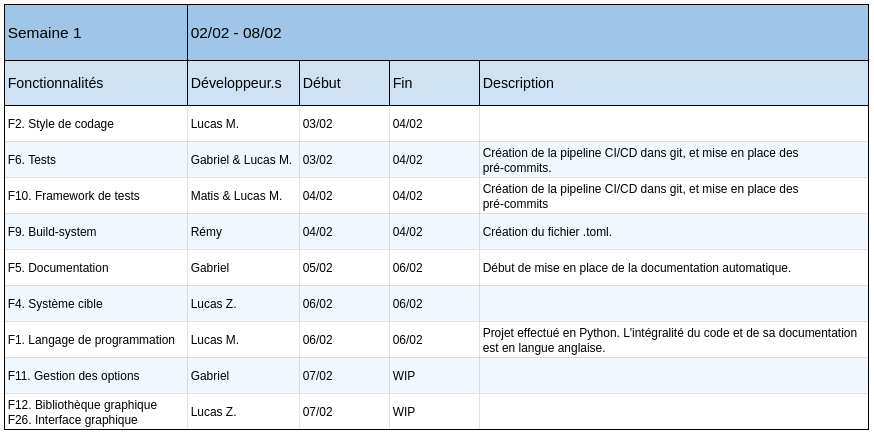
\includegraphics[width=0.9\textwidth]{images/AR_week_01.png}
    \caption{Tâches effectuées pendant la première semaine du projet}
    \title{fig:AR_week_01.png}

    \vspace{1cm}

\end{figure}

\begin{figure}[h]
    \centering
    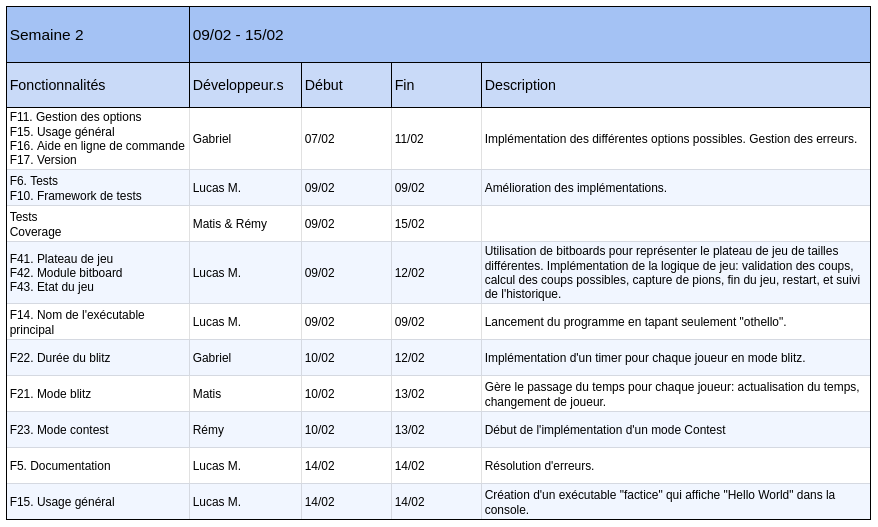
\includegraphics[width=0.9\textwidth]{images/AR_week_02.png}
    \caption{Tâches effectuées pendant la seconde semaine du projet}
    \title{fig:AR_week_0.png}

    \vspace{1cm}

    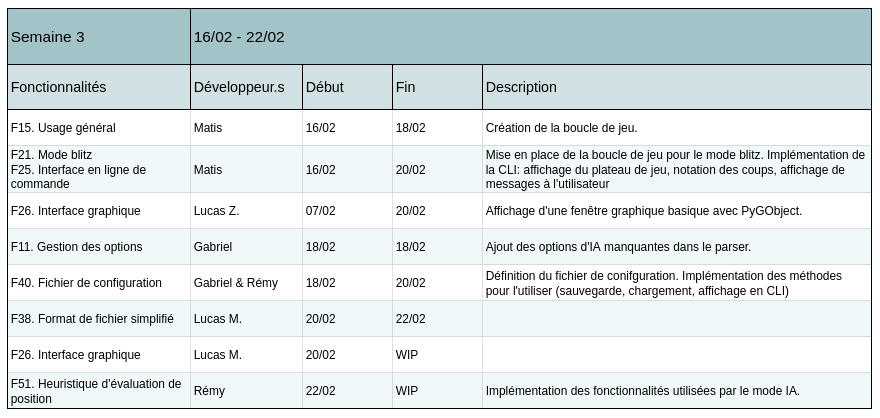
\includegraphics[width=0.9\textwidth]{images/AR_week_03.png}
    \caption{Tâches effectuées pendant la troisième semaine du projet}
    \title{fig:AR_week_0.png}
\end{figure}

\begin{figure}[h]
    \centering
    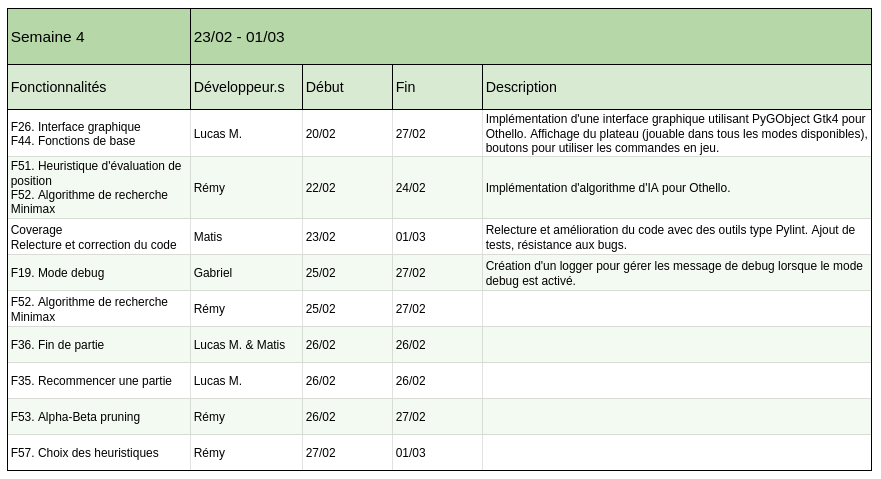
\includegraphics[width=0.9\textwidth]{images/AR_week_04.png}
    \caption{Tâches effectuées pendant la quatrième semaine du projet}
    \title{fig:AR_week_0.png}

    \vspace{1cm}

    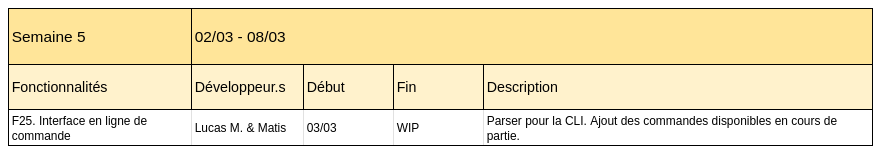
\includegraphics[width=0.9\textwidth]{images/AR_week_05.png}
    \caption{Tâches effectuées pendant la cinquième semaine du projet}
    \title{fig:AR_week_0.png}

    \vspace{1cm}

    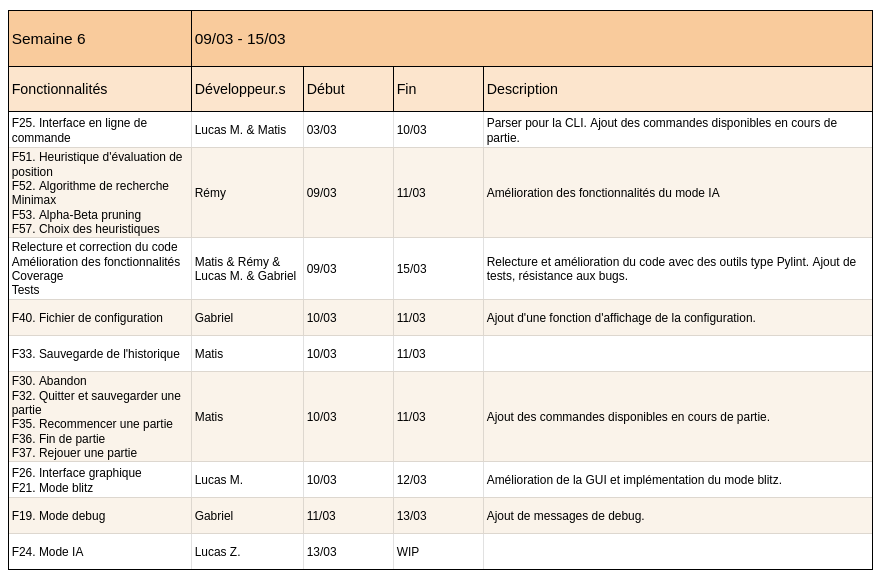
\includegraphics[width=0.9\textwidth]{images/AR_week_06.png}
    \caption{Tâches effectuées pendant la sixième semaine du projet}
    \title{fig:AR_week_0.png}
\end{figure}

\begin{figure}[h]
    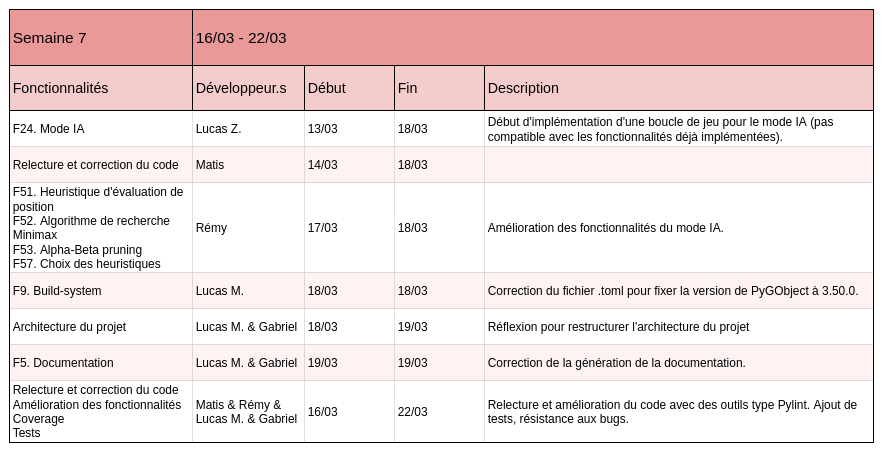
\includegraphics[width=0.9\textwidth]{images/AR_week_07.png}
    \caption{Tâches effectuées pendant la septième semaine du projet}
    \title{fig:AR_week_0.png}

    \vspace{1cm}

    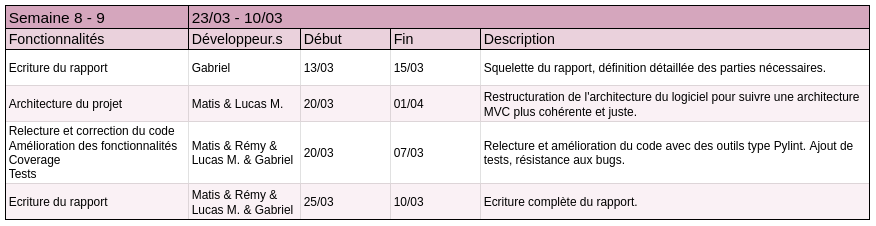
\includegraphics[width=0.9\textwidth]{images/AR_week_08-09.png}
    \caption{Tâches effectuées pendant les huitième et neuvième semaines du projet}
    \title{fig:AR_week_0.png}
\end{figure}

\FloatBarrier

\newpage

\section{Bibliographie}

\bibliographystyle{plainnat}
\bibliography{bibliography}

\end{document}

% \begin{lstlisting}[language=Python, caption=Déclaration de la fonction create_parser]
%     create_parser() -> ArgumentParser
% \end{lstlisting}
